%!TEX TS-program = pdflatex
%!TEX encoding = UTF-8 Unicode
% =============================================================================
%  P1_bernoulli_supp.tex   --  Supplementary Material
%  Compile BEFORE the main paper (see main paper header).
% =============================================================================
\documentclass[bj,authoryear]{imsart}

\usepackage{amsmath,amssymb,mathtools}
\usepackage{bm}
\usepackage{booktabs}
\usepackage{array}
\usepackage{multirow}
\usepackage{enumitem}
\usepackage{graphicx}
\usepackage{float}
\usepackage{nicefrac}
\usepackage{microtype}
\startlocaldefs

\theoremstyle{plain}
\newtheorem{theorem}{Theorem}[section]
\newtheorem{proposition}[theorem]{Proposition}
\newtheorem{lemma}[theorem]{Lemma}
\newtheorem{corollary}[theorem]{Corollary}
\theoremstyle{definition}
\newtheorem{definition}[theorem]{Definition}
\newtheorem{example}[theorem]{Example}
\newtheorem{remark}[theorem]{Remark}
\newtheorem{assumption}[theorem]{Assumption}

\newcommand{\E}{\mathbb{E}}
\newcommand{\Prob}{\mathbb{P}}
\newcommand{\R}{\mathbb{R}}
\newcommand{\N}{\mathbb{N}}
\newcommand{\F}{\mathcal{F}}
\newcommand{\G}{\mathcal{G}}
\newcommand{\A}{\mathcal{A}}
\newcommand{\Z}{\mathbb{Z}}
\newcommand{\Tsig}{\mathcal{T}_\infty}
\newcommand{\norm}[1]{\left\lVert #1 \right\rVert}
\newcommand{\abs}[1]{\left| #1 \right|}
\newcommand{\inner}[2]{\langle #1,\, #2 \rangle}
\newcommand{\given}{\mid}
\newcommand{\iid}{\overset{\mathrm{iid}}{\sim}}
\DeclareMathOperator{\Var}{Var}
\DeclareMathOperator{\Cov}{Cov}
\DeclareMathOperator*{\argmin}{arg\,min}
\newcommand{\od}[1]{\overset{d}{#1}}

\endlocaldefs

%% Cross-references to the companion document are LIVE and SELF-FREEZING.
%% While the companion's .aux is present it is read at compile time (only
%% its \newlabel entries are kept), so renumbering can never go stale, and
%% a snapshot \jobname-xrefs.tex is (re)written automatically on every
%% compile.  When the companion's .aux is absent -- e.g. the journal
%% compiling this file in isolation -- the snapshot is used instead.
%% Submission: upload \jobname-xrefs.tex together with the source, exactly
%% like the .bbl file.  (The xr package is NOT used: imsart forbids it.)
\makeatletter
\newwrite\companion@xrefs@out
\newcommand{\companionlabel}[2]{%
  \global\expandafter\def\csname r@#1\endcsname{#2}}
\def\companion@readaux#1{%
  \immediate\openout\companion@xrefs@out=\jobname-xrefs.tex
  \immediate\write\companion@xrefs@out{%
    \@percentchar\space Snapshot of the cross-references in #1.aux.}%
  \immediate\write\companion@xrefs@out{%
    \@percentchar\space Auto-regenerated on every compile; do not edit.}%
  \begingroup
    \let\citation\@gobble
    \let\bibdata\@gobble
    \let\bibstyle\@gobble
    \def\bibcite##1##2{}%
    \long\def\@writefile##1##2{}%
    \def\newlabel##1##2{%
      \companionlabel{##1}{##2}%
      \immediate\write\companion@xrefs@out{%
        \string\companionlabel{##1}{\unexpanded{##2}}}}%
    \@@input #1.aux\relax
  \endgroup
  \immediate\closeout\companion@xrefs@out}
\def\companion@fallback#1{%
  \IfFileExists{\jobname-xrefs.tex}%
    {\typeout{** #1.aux not found; using frozen snapshot \jobname-xrefs.tex}%
     \input{\jobname-xrefs.tex}}%
    {\typeout{** #1.aux not found and no snapshot; companion refs undefined}}}
\newcommand{\inputcompanionaux}[1]{%
  \IfFileExists{#1.aux}%
    {\companion@readaux{#1}}%
    {\companion@fallback{#1}}}
\inputcompanionaux{P1_bernoulli_20260701_Bernoulli_revised}
\makeatother

% =============================================================================
\begin{document}

\begin{frontmatter}
\title{Supplementary Material for:\\[0.3em]
  Martingale Innovations from Recurrent Networks\\[0.1em]
  for Sequential Change-Point Detection}
\runtitle{Supplementary Material}
\author{\inits{Y.-C.\,I.}\fnms{Yuan-chin Ivan}~\snm{Chang}}
\end{frontmatter}

% Reset section/equation counters to A, B, C style for appendix
\setcounter{section}{0}
\renewcommand{\thesection}{\Alph{section}}
\renewcommand{\theequation}{\Alph{section}.\arabic{equation}}
\renewcommand{\thetable}{\Alph{section}.\arabic{table}}
\renewcommand{\thefigure}{\Alph{section}.\arabic{figure}}
\renewcommand{\thetheorem}{\Alph{section}.\arabic{theorem}}

% =============================================================================
\section{Background and Preliminaries}
\label{app:background}

We work throughout on a complete probability space $(\Omega, \A, \Prob)$.
All convergence statements are in the almost-sure or $L^p$ sense unless otherwise noted.

\subsection{Filtrations and the Information Flow}

\begin{definition}[Filtration and natural filtration]
\label{def:filtration}
  A \emph{filtration} is an increasing family of sub-$\sigma$-algebras
  $\F_1 \subseteq \F_2 \subseteq \cdots \subseteq \A$.
  For a sequence $(X_t)_{t\geq 1}$ of random variables, the
  \emph{natural filtration} is $\F_t = \sigma(X_1, \ldots, X_t)$ and its
  completion $\F_\infty^+ = \sigma\bigl(\bigcup_{t\geq 1}\F_t\bigr)$.
\end{definition}

A \emph{decreasing filtration} (or \emph{reverse filtration}) is a family
$\G_1 \supseteq \G_2 \supseteq \cdots$ of sub-$\sigma$-algebras.
The canonical example relevant to this paper is
\begin{equation}
  \G_n = \sigma(X_n, X_{n+1}, \ldots),
  \label{eq:reverse-filtration}
\end{equation}
which formalizes the information contained in the \emph{tail} of the sequence
starting at index $n$.

\begin{definition}[Tail $\sigma$-algebra]
\label{def:tail}
  The \emph{tail $\sigma$-algebra} of a sequence $(X_t)_{t\geq 1}$ is
  \[
    \Tsig = \bigcap_{n=1}^\infty \sigma(X_n, X_{n+1}, \ldots)
           = \bigcap_{n=1}^\infty \G_n.
  \]
  An event $A \in \Tsig$ is \emph{tail-measurable}: its occurrence or
  non-occurrence is not affected by any finite initial segment of the sequence.
\end{definition}

\begin{example}[Tail-measurable functionals]
  For an i.i.d.\ or ergodic sequence $(X_t)$:
  (a) the limit $\lim_{n\to\infty} n^{-1}\sum_{t=1}^n X_t$ (when it exists)
      is $\Tsig$-measurable;
  (b) the event $\{\limsup_{t\to\infty} X_t > c\}$ is tail-measurable;
  (c) the population mean $\mu = \E[X_1]$ is a constant, hence trivially
      $\Tsig$-measurable under any probability measure.
  Finite-dimensional functions of $(X_1,\ldots,X_k)$ for fixed $k$ are
  \emph{not} tail-measurable in general.
\end{example}

\subsection{Martingales and Reverse Martingales}

\begin{definition}[Martingale and martingale difference sequence]
\label{def:martingale}
  A sequence $(M_t, \F_t)_{t\geq 1}$ is a \emph{martingale} if
  $\E[\abs{M_t}] < \infty$ and $\E[M_{t+1}\given\F_t] = M_t$ a.s.\ for all $t$.
  The sequence $(D_t)_{t\geq 1}$ is a \emph{martingale difference sequence} (MDS)
  if $\E[\abs{D_t}] < \infty$ and $\E[D_t\given\F_{t-1}] = 0$ a.s.\ for all $t\geq 2$.
\end{definition}

The posterior mean $\E[\theta\given\F_t]$, for a fixed integrable parameter
$\theta$ and observations $X_1, X_2, \ldots$, is the canonical martingale in
Bayesian sequential analysis.

\begin{definition}[Reverse martingale]
\label{def:reverse-mg}
  Let $(\G_n)_{n\geq 1}$ be a decreasing filtration.
  A sequence $(Y_n, \G_n)_{n\geq 1}$ is a \emph{reverse martingale} if
  $\E[\abs{Y_n}] < \infty$ and
  \[
    \E[Y_n \given \G_{n+1}] = Y_{n+1} \quad \text{a.s.\ for all } n\geq 1.
  \]
\end{definition}

A prototypical reverse martingale is obtained by taking an integrable random
variable $Y$ and setting $Y_n=\E[Y\mid\G_n]$ for a decreasing filtration
$(\G_n)$.  Exchangeability arguments also represent empirical averages through
appropriate decreasing sigma-fields.  The key convergence theorem is:

\begin{theorem}[Reverse martingale convergence; \citealt{doob1953stochastic}]
\label{thm:revmg}
  If $(Y_n, \G_n)_{n\geq 1}$ is an $L^1$-bounded reverse martingale with
  decreasing filtration $(\G_n)$, then
  \[
    Y_n \xrightarrow{a.s.\ \text{and}\ L^1}
    Y_\infty := \E\!\left[Y_1 \,\middle|\, \G_\infty\right],
    \qquad \G_\infty = \bigcap_{n \geq 1} \G_n.
  \]
\end{theorem}

\begin{proof}
  Let $(Y_n, \G_n)_{n\geq 1}$ be an $L^1$-bounded reverse martingale
  with decreasing filtration $\G_1 \supseteq \G_2 \supseteq \cdots$
  and $\G_\infty = \bigcap_{n\geq 1}\G_n$.
  Without loss of generality, write $Y_n = \E[Y_1\given\G_n]$, which is
  consistent with the reverse martingale property by the tower law:
  for $m > n$, $\G_m \subseteq \G_n$ implies
  $\E[Y_n\given\G_m] = \E[\E[Y_1\given\G_n]\given\G_m]
   = \E[Y_1\given\G_m] = Y_m$ a.s.

  \textbf{Almost-sure convergence.}
  For any $a < b$, let $U_n([a,b])$ be the number of upcrossings of
  $[a,b]$ by the sequence $Y_1, Y_2, \ldots, Y_n$.
  Doob's upcrossing inequality for reverse martingales
  \citep[Chapter~V]{neveu1975discrete} gives
  \[
    (b-a)\,\E[U_n([a,b])] \leq \E[(Y_1 - a)^+] \leq \E[|Y_1|] + |a| < \infty.
  \]
  Letting $n\to\infty$, the monotone convergence theorem gives
  $\E[U_\infty([a,b])] < \infty$, so $U_\infty([a,b]) < \infty$ a.s.
  Since $a < b$ are arbitrary rationals, the number of upcrossings of
  every rational interval is finite almost surely, which implies
  $Y_n \to Y_\infty$ a.s.\ for some $[-\infty,\infty]$-valued random
  variable $Y_\infty$.

  \textbf{$L^1$ convergence and integrability of the limit.}
  For each $n$, $|Y_n| = |\E[Y_1\given\G_n]| \leq \E[|Y_1|\given\G_n]$
  by Jensen's inequality.  The family $\{\E[|Y_1|\given\G_n]\}_{n\geq 1}$
  is uniformly integrable by the standard fact that the collection of
  conditional expectations $\{\E[Z\given\G] : \G \subseteq \A\}$ of a
  fixed $Z \in L^1$ is uniformly integrable
  \citep[Sec.~13.4]{williams1991probability}.
  Hence $\{Y_n\}$ is uniformly integrable.
  Uniform integrability together with a.s.\ convergence implies $L^1$
  convergence: $\norm{Y_n - Y_\infty}_{L^1} \to 0$, and in particular
  $Y_\infty \in L^1$.

  \textbf{Identification of the limit.}
  For any $A \in \G_\infty \subseteq \G_n$, the definition of conditional
  expectation gives $\int_A Y_n\,d\Prob = \int_A Y_1\,d\Prob$ for all
  $n$.  Passing to the limit using $L^1$ convergence:
  $\int_A Y_\infty\,d\Prob = \int_A Y_1\,d\Prob$ for all $A\in\G_\infty$.
  By the definition of conditional expectation,
  $Y_\infty = \E[Y_1\given\G_\infty]$ a.s.
\end{proof}

\begin{remark}[Comparison with forward convergence]
  Doob's \emph{forward} martingale convergence theorem requires $L^1$-boundedness
  and yields almost-sure convergence but not necessarily $L^1$ convergence
  (unless the martingale is uniformly integrable).
  Reverse martingales are automatically uniformly integrable, so both modes of
  convergence are free.  This property is useful for tail-projection arguments such as
  Lemma~\ref{lem:equiv} of the main paper.
\end{remark}

\subsection{The Hewitt--Savage Zero-One Law}
\label{app:hw}

\begin{theorem}[Hewitt--Savage; \citealt{hewitt1955symmetric}]
\label{thm:hs}
  Let $(X_t)_{t\geq 1}$ be an i.i.d.\ sequence.  Then every event invariant
  under finite permutations of the coordinates has probability $0$ or $1$.
  In particular, every tail event $A\in\Tsig$ satisfies
  $\Prob(A)\in\{0,1\}$.
\end{theorem}

For i.i.d.\ sequences, Theorem~\ref{thm:hs} implies that the tail
$\sigma$-algebra is trivial, so $\E[Z\given\Tsig]=\E[Z]$ for any integrable
$Z$.  The statement should not be extended to arbitrary exchangeable sequences:
by de Finetti's theorem, an exchangeable but non-i.i.d.\ Bernoulli sequence can
have a nontrivial tail generated by the random mixing parameter.  For stationary
ergodic sequences, the ergodic theorem identifies limits of time averages, but
it does not imply that every tail-measurable functional is literally a time
average.

\subsection{Recurrent Neural Networks and LSTMs}

We give precise definitions of the two architectures whose hidden states we analyze.

\begin{definition}[Recurrent Neural Network]
\label{def:rnn}
  An \emph{RNN} processes a sequence $(x_t)_{t=1}^T$, $x_t \in \R^p$, via
  \begin{equation}
    h_t = \phi(W_h h_{t-1} + W_x x_t + b_h),
    \label{eq:rnn}
  \end{equation}
  where $h_t \in \R^d$ is the \emph{hidden state}, $W_h \in \R^{d\times d}$,
  $W_x \in \R^{d\times p}$, $b_h \in \R^d$, and $\phi:\R^d\to\R^d$ is a
  coordinate-wise non-linear activation (e.g.\ $\tanh$ or ReLU).
  The initial state $h_0 \in \R^d$ is fixed or learnable; the $L^2$ theory below assumes it is square-integrable.
\end{definition}

\begin{remark}[Notation]
  In this appendix $d$ denotes the hidden-state dimension and $p$ the input dimension.
  In the main paper (Section~2), the same dimensions are written $p$ (hidden) and $d_{\mathrm{in}}$ (input); the symbol $d$ in the main paper refers to the observation dimension in the empirical studies (Section~4).
\end{remark}

\begin{assumption}[Effective operator-norm contractivity, restated]
\label{ass:spectral-supp}
  This restates the main paper's contractivity assumption for the reader's
  convenience; it is not a separate hypothesis.  Throughout the paper we
  assume
  \[
    L_\phi\norm{W_h}_{\mathrm{op}}<1,
  \]
  where $L_\phi$ is the Lipschitz constant of the activation $\phi$ and
  $\norm{W_h}_{\mathrm{op}}=\sigma_{\max}(W_h)$ is the operator norm.  This is
  the contraction needed for $L^2$-stability of~\eqref{eq:rnn}.  The spectral
  radius alone is insufficient for non-normal matrices because it does not
  control the vector norm.  Spectral normalization can encourage or enforce this
  condition after accounting for $L_\phi$ \citep{miyato2018spectral}.
\end{assumption}

\begin{definition}[Long Short-Term Memory]
\label{def:lstm}
  An \emph{LSTM} \citep{hochreiter1997long} augments the basic RNN with a cell
  state $c_t \in \R^d$ and three gating mechanisms:
  \begin{align}
    f_t &= \sigma(W_f [h_{t-1}; x_t] + b_f), \label{eq:forget}\\
    i_t &= \sigma(W_i [h_{t-1}; x_t] + b_i), \label{eq:input}\\
    o_t &= \sigma(W_o [h_{t-1}; x_t] + b_o), \label{eq:output-gate}\\
    \tilde{c}_t &= \tanh(W_c [h_{t-1}; x_t] + b_c), \label{eq:candidate}\\
    c_t &= f_t \odot c_{t-1} + i_t \odot \tilde{c}_t, \label{eq:cell}\\
    h_t &= o_t \odot \tanh(c_t), \label{eq:hidden}
  \end{align}
  where $[h_{t-1};x_t]\in\R^{d+p}$ denotes concatenation, $\sigma$ is the
  logistic sigmoid, and $\odot$ is coordinate-wise multiplication.
  The \emph{forget gate} $f_t \in (0,1)^d$ controls how much of the previous
  cell state survives to time $t$.
\end{definition}

\begin{remark}[Contractivity of LSTM]
  The coordinate-wise bound $f_t\in(0,1)^d$ does not by itself make the full
  LSTM cell recursion uniformly contractive.  The gate can be arbitrarily close
  to one, and $f_t$ depends on $h_{t-1}$, which depends on $c_{t-1}$, so
  derivatives of the gate map also enter the Lipschitz constant.  A rigorous
  contraction theorem for LSTMs therefore requires a separate assumption, such
  as a uniform gate bound $\norm{f_t}_\infty\leq\gamma<1$ together with Lipschitz
  control of the gate maps.  In this paper, the rigorous contraction theorem is
  stated only for the basic RNN recurrence.
\end{remark}

\subsection{Stationary Ergodic Processes}

\begin{definition}[Stationarity and ergodicity]
\label{def:ergodic}
  A process $(X_t)_{t\geq 1}$ is \emph{(strictly) stationary} if
  $$(X_{t+k})_{t\geq 1} \overset{d}{=} (X_t)_{t\geq 1}$$ for all $k \geq 1$.
  It is \emph{ergodic} if every shift-invariant event has probability 0 or 1.
  By the ergodic theorem \citep{walters2000introduction}, for any $L^1$
  functional $g$,
  \[
    \frac{1}{T}\sum_{t=1}^T g(X_t) \xrightarrow{a.s.} \E[g(X_1)]
    \quad \text{as } T\to\infty.
  \]
\end{definition}

Stationarity is the maintained assumption throughout the theory sections
(Sections~\ref{sec:theory}--\ref{sec:pathway}) of the main paper;
the empirical Section~\ref{sec:empirical} deliberately includes non-stationary
change-point and real-data settings.  The non-stationary extension via locally
stationary processes \citep{dahlhaus1997fitting} is treated in
Section~\ref{sec:nonstationary} of the main paper.

% =============================================================================
\section{Proofs}
\label{app:proofs}

For reference, Table~\ref{tab:assumption-map} maps each result of the main
paper to the object it concerns, the assumptions it requires, and what it
establishes; the proofs follow in order.

\begin{table}[ht]
\centering
\footnotesize
\caption{Map of the main-paper results.  The top block (tier one) concerns
  the contractive RNN and its innovations; the bottom block (tier two)
  concerns the Innovation CUSUM detector and requires no RNN contraction
  theorem, only conditional residual-drift and tail conditions on
  fitted residuals.}
\label{tab:assumption-map}
\renewcommand{\arraystretch}{1.2}
\begin{tabular}{@{}l p{2.3cm} p{4.0cm} p{3.4cm}@{}}
\toprule
Result & Object & Key assumptions & Establishes \\
\midrule
Thm~\ref{thm:mds} & Contractive RNN state $h_t$
  & stationary ergodic input, $\E\norm{X}^2<\infty$,
    $L_\phi\norm{W_h}_{\mathrm{op}}<1$
  & Doob/MDS decomposition; geometric innovation stabilization \\
Cor~\ref{cor:fclt} & RNN innovations $M_t$
  & additionally $(2{+}\delta)$-moment, $\Sigma_M^*\succ0$
  & functional CLT for cumulative innovations \\
Prop~\ref{prop:predresid} & Prediction residuals $e_t$
  & Bayes predictor (exact); $L^2$-accurate fitted predictor (approx.)
  & exact / approximate MDS \\
Prop~\ref{prop:rnn-resid-bridge} & Recurrent predictor residuals
  & hypotheses of Thm~\ref{thm:mds}; Lipschitz readout
  & residual drift $\leq L_o\rho^t\Delta_0$ $+$ stationary readout error \\
Prop~\ref{prop:whiteness} & Fitted vs.\ linear residuals
  & nonlinear conditional mean; consistent learned predictor
  & irreducible linear defect; learned defect $\to0$ \\
Prop~\ref{prop:whiteness-rate} & Fitted-predictor defect $\eta_T$
  & approximation rate $W^{-2\beta}$; $\beta$-mixing excess-risk rate
  & $\eta_T=\widetilde O(T^{-\beta/(2\beta+1)})$; margin $\kappa_T\uparrow k$ \\
\midrule
Thm~\ref{thm:arl} & Innovation CUSUM score
  & drift margin $k>\eta$, conditional sub-Gaussianity
  & exponential in-control ARL lower bound \\
Thm~\ref{thm:delay} & Innovation CUSUM score
  & post-change drift $\geq k+\mu$, bounded increments
  & out-of-control detection-delay upper bound \\
Cor~\ref{cor:tradeoff} & Innovation CUSUM score
  & Assumptions above
  & exponential-ARL / logarithmic-delay trade-off \\
Thm~\ref{thm:optimality} & Innovation CUSUM score
  & Assumptions above; Gaussian innovation shift for exactness
  & Lorden order-optimality; exact minimax optimality (Gaussian) \\
Cor~\ref{cor:dim} & Mahalanobis innovation score
  & uniform-in-$d$: bounded $\eta_d$, $\lambda_{\min}(\Sigma_0)\ge c_0$,
    conditional homoskedasticity, $O(1)$ score sub-Gaussianity
  & dimension-stable ARL \\
\bottomrule
\end{tabular}
\end{table}

\subsection{Proof of Lemma~\ref{lem:equiv} of the main paper (Equivalence of Forward and Tail Limits)}
\label{app:proof-lemequiv}

\begin{proof}[Proof of Lemma~\ref{lem:equiv} in the main paper]
  \textbf{Part (a).}
  Since $\theta \in L^\infty \subseteq L^1$ and $\theta$ is
  $\Tsig$-measurable, it is also $\F_\infty^+$-measurable because
  $\Tsig \subseteq \G_1 = \sigma(X_1,X_2,\ldots) \subseteq \F_\infty^+$.
  By Doob's $L^1$ martingale convergence theorem \citep{doob1953stochastic},
  $\E[\theta\given\F_t] \to \E[\theta\given\F_\infty^+]$ a.s.\ and in $L^1$.
  Since $\theta$ is $\F_\infty^+$-measurable,
  $\E[\theta\given\F_\infty^+] = \theta$ a.s.

  \textbf{Part (b).}
  The sequence $(\E[\theta\given\G_n], \G_n)_{n\geq 1}$ is a reverse
  martingale: for $m > n$, $\G_m \subseteq \G_n$ implies
  $\E[\E[\theta\given\G_n]\given\G_m] = \E[\theta\given\G_m]$ by the
  tower property.
  Boundedness of $\theta$ gives $L^1$-boundedness.
  By the reverse martingale convergence theorem
  (Theorem~\ref{thm:revmg}; \citealt{doob1953stochastic}),
  $\E[\theta\given\G_n] \to \E[\theta\given\Tsig]$ a.s.\ and in $L^1$.
  Since $\theta$ is $\Tsig$-measurable, $\E[\theta\given\Tsig] = \theta$
  a.s.

  \textbf{Part (c).}
  Immediate from (a) and (b): both limits equal $\theta$ a.s.

  \textbf{Parts (d) and (e).}
  For general $\theta \in L^1$, part (a) extends to
  $\E[\theta\given\F_t]\to\E[\theta\given\F_\infty^+]$ by the same Doob
  argument.  For part (e), the reverse martingale convergence in (b)
  applies unchanged since the reverse martingale is
  $(\E[\theta\given\G_n], \G_n)$, and the limit is
  $\E[\theta\given\Tsig]$ regardless of whether $\theta$ is
  tail-measurable.  The two limits agree if and only if
  $\E[\theta\given\F_\infty^+]$ is $\Tsig$-measurable, which holds when
  $\theta$ itself is tail-measurable.
\end{proof}

\subsection{Proof of Theorem~\ref{thm:mds} of the main paper (MDS Decomposition with Stabilization Rate)}
\label{app:proof-thmmds}

\begin{proof}[Proof of Theorem~\ref{thm:mds} in the main paper]
  Throughout, $\rho = L_\phi\norm{W_h}_{\mathrm{op}} < 1$ and
  $\Delta_0 = \norm{h_0 - H_0^*}_{L^2}$.

  \textbf{Part (i): $L^2$-boundedness.}
  We prove the $C_0$ formula for the case $\phi(0)=0$ (e.g.\ $\tanh$, ReLU),
  where the Lipschitz bound gives $\norm{\phi(u)} \leq L_\phi\norm{u}$.
  (For activations with $\phi(0)\neq 0$, e.g.\ sigmoid, an additional
  term $L_\phi\norm{\phi(0)}/(1-\rho)$ is added to $C_0$, consistent with the
  general formula stated in Theorem~\ref{thm:mds} of the main paper.)
  By the Lipschitz bound $\norm{\phi(u)}\leq L_\phi\norm{u}$ and
  Minkowski's inequality in $L^2$,
  \[
    \norm{h_t}_{L^2}
    \leq L_\phi\norm{W_hh_{t-1}+W_xX_t+b_h}_{L^2}
    \leq \rho\norm{h_{t-1}}_{L^2}
      + L_\phi\norm{W_x}_{\mathrm{op}}\norm{X_t}_{L^2}
      + L_\phi\norm{b_h}.
  \]
  Let $c := L_\phi(\norm{W_x}_{\mathrm{op}}\norm{X_1}_{L^2}+\norm{b_h})$,
  which is finite by stationarity.  Iterating the inequality and summing
  the geometric series gives
  \[
    \norm{h_t}_{L^2} \leq \rho^t\norm{h_0}_{L^2} + \frac{c}{1-\rho},
  \]
  so $\sup_t\norm{h_t}_{L^2} \leq \norm{h_0}_{L^2} + c/(1-\rho) =: C_0 < \infty$.

  \textbf{Part (ii): MDS structure.}
  Since $h_t$ is $\F_t$-measurable and square-integrable by part~(i),
  the conditional expectation $D_t := \E[h_t\given\F_{t-1}]$ is
  well-defined and $\F_{t-1}$-measurable.  Setting $M_t := h_t - D_t$,
  \[
    \E[M_t\given\F_{t-1}]
    = \E[h_t - D_t\given\F_{t-1}]
    = D_t - D_t = 0 \quad\text{a.s.}
  \]

  \textbf{Part (iii): Innovation $L^2$ bound.}
  Conditional on $\F_{t-1}$, the previous state $h_{t-1}$ is fixed and
  the only new random input is $X_t$.  Put $\mu_t = \E[X_t\mid\F_{t-1}]$
  and define $g_t(x) := \phi(W_h h_{t-1} + W_x x + b_h)$.
  Since $h_{t-1}$ is $\F_{t-1}$-measurable, $g_t(\mu_t) = \phi(W_hh_{t-1}+W_x\mu_t+b_h)$ is $\F_{t-1}$-measurable.
  By the best-approximation property of the conditional expectation ($D_t = \E[h_t|\F_{t-1}]$ minimizes the $L^2$ distance to $h_t$ over all $\F_{t-1}$-measurable functions),
  \begin{align*}
    \E\bigl\{\norm{M_t}^2\mid\F_{t-1}\bigr\}
    &\leq \E\bigl\{\norm{g_t(X_t) - g_t(\mu_t)}^2\mid\F_{t-1}\bigr\} \\
    &\leq L_\phi^2\norm{W_x}_{\mathrm{op}}^2\,
           \E\bigl\{\norm{X_t - \mu_t}^2\mid\F_{t-1}\bigr\}.
  \end{align*}
  Taking unconditional expectations: since
  $\E\{\norm{X_t-\mu_t}^2\mid\F_{t-1}\} = \Var(X_t\mid\F_{t-1})$ is the
  conditional variance, the law of total variance gives
  $\E[\Var(X_t\mid\F_{t-1})] = \Var_2(X_t) - \E\norm{\mu_t-\E X_t}^2
    \leq \Var_2(X_t)$,
  which yields equation~\eqref{eq:Mbound} in the main paper.

  \textbf{Part (iv): Innovation stabilization rate.}
  Write $M_t - M_t^* = (h_t - H_t^*) - (D_t - D_t^*)$.
  By the triangle inequality,
  $\norm{M_t - M_t^*}_{L^2}
  \leq \norm{h_t - H_t^*}_{L^2} + \norm{D_t - D_t^*}_{L^2}$.
  The coupling bound (Proposition~\ref{prop:stationary-causal} below) gives
  $\norm{h_t - H_t^*}_{L^2} \leq \rho^t\Delta_0$.
  Since conditional expectation is an $L^2$ contraction,
  $\norm{D_t - D_t^*}_{L^2}
  = \norm{\E[h_t - H_t^*\mid\F_{t-1}]}_{L^2}
  \leq \norm{h_t - H_t^*}_{L^2}
  \leq \rho^t\Delta_0$.
  Adding the two bounds gives $\norm{M_t - M_t^*}_{L^2} \leq 2\rho^t\Delta_0$.

  \textbf{Part (v): Variance decomposition and $\Sigma_M^*$.}
  The law of total variance applied coordinatewise, combined with
  $\E[M_t\given\F_{t-1}] = 0$, gives
  \[
    \E\norm{h_t - \E h_t}^2
    = \E\norm{D_t - \E h_t}^2 + \E\norm{M_t}^2,
  \]
  since the cross term $2\E\langle D_t - \E h_t,\, M_t\rangle = 0$.

  For the stationary regime, recall that the filtration is the two-sided
  past $\F_{t-1} = \sigma(X_s : s\leq t-1)\vee\sigma(h_0)$ with $h_0$
  independent of the process (main paper, Section~2 setup).  By the causal
  construction (Proposition~\ref{prop:stationary-causal}), $H_t^*$ is the
  same fixed measurable functional of $(\ldots,X_{t-1},X_t)$ at every $t$,
  and since $\sigma(h_0)$ is independent of $\sigma(X_s: s\in\Z)$,
  conditioning on it leaves the conditional expectation unchanged:
  $D_t^* = \E[H_t^*\given\F_{t-1}]
   = \E[H_t^*\given\sigma(X_s:s\leq t-1)]$
  is likewise the same functional of the shifted path at every $t$.
  Hence $(M_t^* = H_t^* - D_t^*)_{t\in\Z}$ is strictly stationary and
  $\Sigma_M^* := \E[M_t^*(M_t^*)^\top]$ is independent of $t$.
  (With the one-sided filtration $\sigma(X_1,\ldots,X_{t-1})$ this would
  fail: the conditioning set is not shift-invariant.)
  Positive semi-definiteness is immediate.  The bound
  $\Sigma_M^* \preceq \sigma_M^2 I_p$ follows from part~(iii) applied to the
  stationary solution: for a positive semi-definite matrix,
  $\lambda_{\max}(\Sigma_M^*) \leq \mathrm{tr}(\Sigma_M^*)
   = \E\norm{M_t^*}^2 \leq \sigma_M^2$.

  For strict positivity of $\Sigma_M^*$: suppose for contradiction that
  $\lambda_{\min}(\Sigma_M^*) = 0$.  Then there exists a unit vector
  $v\in\R^p$ with $\E[(v^\top M_t^*)^2] = 0$, so $v^\top M_t^* = 0$ a.s.,
  meaning $v^\top H_t^*$ is $\F_{t-1}$-measurable.  But then
  $\Var(v^\top H_t^*\mid\F_{t-1}) = 0$ a.s., which contradicts the
  nondegeneracy condition~(5) in the main paper
  (equation~\eqref{eq:nondeg}: $\Var(v^\top\phi(W_hH_{t-1}^*+W_xX_t+b_h)\mid\F_{t-1})>0$
  a.s.\ for all nonzero $v$).
  Hence $\lambda_{\min}(\Sigma_M^*)>0$ under that condition.

  \emph{Remark on the full row rank sufficient condition.}
  A classical sufficient condition for equation~\eqref{eq:nondeg} is
  $\mathrm{rank}(W_x)=p$ together with $X_t$ not entirely predictable
  from $\F_{t-1}$.  When $W_x$ has full row rank,
  $W_x^\top v\neq0$ for all nonzero $v$, which implies
  $\Var(v^\top H_t^*\mid\F_{t-1})>0$ a.s.\ for all nonzero $v$ under \emph{linear} activation (so that variance propagates linearly through $g_t$).
  This implication can fail for nonlinear $\phi$ in a nearly flat or saturating region; the nondegeneracy condition~\eqref{eq:nondeg}
  is the correct sufficient condition in general.
\end{proof}

\subsection{Proof of Corollary~\ref{cor:fclt} of the main paper (Functional CLT for MDS Innovations)}
\label{app:proof-corfclt}

\begin{proof}[Proof of Corollary~\ref{cor:fclt} in the main paper]
  \textbf{CLT for the stationary process $(M_t^*)$.}
  Under the two-sided filtration
  $\F_t = \sigma(X_s:s\leq t)\vee\sigma(h_0)$ of the main-paper setup,
  $H_t^*$ --- and hence $M_t^* = H_t^* - \E[H_t^*\given\F_{t-1}]$ --- is
  $\F_t$-measurable by the causal construction, so
  $(M_t^*, \F_t)_{t\geq 1}$ is an \emph{adapted}, strictly stationary MDS
  (stationarity by the proof of Theorem~\ref{thm:mds}(v) above); the
  martingale FCLT below requires this adaptedness.
  We verify $\sup_t\E\norm{M_t^*}^{2+\delta}<\infty$.
  By the Lipschitz recursion and Minkowski's inequality in $L^{2+\delta}$,
  \[
    \norm{H_t^*}_{L^{2+\delta}}
    \leq \rho\norm{H_{t-1}^*}_{L^{2+\delta}}
       + L_\phi\norm{W_x}_{\mathrm{op}}\norm{X_t}_{L^{2+\delta}}
       + L_\phi\norm{b_h}.
  \]
  Stationarity gives a common value $C = c'/(1-\rho) < \infty$, so $\sup_t\norm{H_t^*}_{L^{2+\delta}} \leq C$.
  Since $D_t^* = \E[H_t^*\given\F_{t-1}]$ and conditional expectation is an $L^{2+\delta}$ contraction,
  $\norm{M_t^*}_{L^{2+\delta}} = \norm{H_t^* - D_t^*}_{L^{2+\delta}} \leq \norm{H_t^*}_{L^{2+\delta}} + \norm{D_t^*}_{L^{2+\delta}} \leq 2C$,
  so $\sup_t\E\norm{M_t^*}^{2+\delta} \leq (2C)^{2+\delta} < \infty$.
  Since $(H_t^*, M_t^*)$ is a measurable function of $(X_t, X_{t-1}, \ldots)$ via the causal representation of Theorem~\ref{thm:mds} in the main paper, and $(X_t)$ is strictly stationary ergodic, the joint process $(H_t^*, M_t^*, X_t)$ is also strictly stationary and ergodic.
  The conditional covariance
  $\E[M_t^*(M_t^*)^\top\given\F_{t-1}]$ is itself a fixed $L^1$ functional
  of the shifted path $(\ldots,X_{t-2},X_{t-1})$, so Birkhoff's ergodic
  theorem, applied to the shift on the path space of $(X_t)_{t\in\Z}$
  (not merely to functions of a single coordinate), gives
  $\frac{1}{T}\sum_{t=1}^T\E[M_t^*(M_t^*)^\top\given\F_{t-1}] \xrightarrow{a.s.} \Sigma_M^*$.
  The conditional Lindeberg condition holds because $C_{2+\delta}:=\E\norm{M_0^*}^{2+\delta}<\infty$:
  by the $L^{2+\delta}$ bound and Markov's inequality,
  \[
    \E\!\left[\frac{1}{T}\sum_{t=1}^T
    \E\!\left[\norm{M_t^*}^2\,\mathbf{1}\{\norm{M_t^*}>\varepsilon\sqrt{T}\}
       \given\F_{t-1}\right]\right]
    \leq \frac{C_{2+\delta}}{(\varepsilon\sqrt{T})^\delta} = O(T^{-\delta/2}) \to 0,
  \]
  so the conditional Lindeberg sum converges to zero in $L^1$ and hence in probability.
  The functional CLT for stationary square-integrable scalar MDS arrays
  \citep[Theorem~4.1]{hall1980martingale} applies coordinate-wise; convergence
  in $\R^p$ follows from the Cram\'er--Wold device.
  Tightness in $D([0,1],\R^p)$ follows from the uniform $L^{2+\delta}$ bound
  via \citet[Theorem~13.5]{billingsley1999convergence}: by the
  Burkholder--Davis--Gundy (BDG) inequality and Jensen's inequality,
  for $0\leq s\leq t\leq 1$ with $n:=\lfloor Tt\rfloor-\lfloor Ts\rfloor$,
  \begin{align*}
    \E\|\mathbf{S}_T(t)-\mathbf{S}_T(s)\|^{2+\delta}
    &\leq C_\delta\,T^{-(2+\delta)/2}\,n^{\delta/2}
        \sum_{j=\lfloor Ts\rfloor+1}^{\lfloor Tt\rfloor}\E\|M_j^*\|^{2+\delta}
    \leq C_\delta C_{2+\delta}\,|t-s|^{1+\delta/2},
  \end{align*}
  where the exponent $\beta = 1 + \delta/2 > 1$ satisfies the requirement
  of Theorem~13.5 (Theorem~15.6 in the 1968 first edition).
  (The displayed bound uses $n\leq 2T|t-s|$, valid for $|t-s|\geq 1/T$;
  increments over gaps shorter than $1/T$ contain at most one summand and
  are handled by the standard partial-sum adjustment, e.g.\
  \citealt[Sec.~13]{billingsley1999convergence}.)  Together these give
  \[
    \frac{1}{\sqrt{T}}\sum_{t=1}^{\lfloor Tu\rfloor} M_t^*
    \xrightarrow{d} (\Sigma_M^*)^{1/2}\,W(u)
    \quad\text{in }D([0,1],\R^p).
  \]

  \textbf{Transient correction.}
  By Theorem~\ref{thm:mds}(iv) of the main paper,
  $\norm{M_t - M_t^*}_{L^2} \leq 2\rho^t\Delta_0$.
  Let $\mathbf{T}_T(u) := T^{-1/2}\sum_{t=1}^{\lfloor Tu\rfloor}(M_t - M_t^*)$.
  By the $L^1$-$L^2$ bound and geometric series,
  \[
    \E\!\left[\sup_{u\in[0,1]}\norm{\mathbf{T}_T(u)}\right]
    \leq \frac{1}{\sqrt{T}}\sum_{t=1}^{\infty}2\rho^t\Delta_0
    = \frac{2\rho\Delta_0}{\sqrt{T}(1-\rho)} \to 0.
  \]
  By Markov's inequality, $\mathbf{T}_T \to 0$ in probability in $D([0,1],\R^p)$,
  and the functional Slutsky theorem completes the proof.
\end{proof}

\subsection{Proof of Proposition~\ref{prop:predresid} of the main paper (Bayes Residuals are MDS)}
\label{app:proof-propresid}

\begin{proof}[Proof of Proposition~\ref{prop:predresid} in the main paper]
  The exact statement follows immediately from the defining property of
  conditional expectation:
  $\E[e_{t+1}\given\F_t]
    = \E[Y_{t+1} - \E(Y_{t+1}\mid\F_t)\mid\F_t] = 0$.
  For fitted residuals $\hat{e}_{t+1} = Y_{t+1} - \hat{m}_t$:
  \[
    \E[\hat{e}_{t+1}\mid\F_t]
    = \E[Y_{t+1} - m_t\mid\F_t] + m_t - \hat{m}_t
    = m_t - \hat{m}_t,
  \]
  and the $L^2$ bound follows from $\sup_t\norm{\hat{m}_t - m_t}_{L^2} \leq \eta$.
\end{proof}

\subsection{Proof of Proposition~\ref{prop:rnn-resid-bridge} of the main paper (Bridge from Recurrent States to Prediction Innovations)}
\label{app:proof-bridge}

\begin{proof}[Proof of Proposition~\ref{prop:rnn-resid-bridge} in the main paper]
  By the triangle inequality and Lipschitz continuity of $o$,
  \[
    \norm{o(h_t)-m_t}_{L^2}
    \leq
    \norm{o(h_t)-o(H_t^*)}_{L^2}
    +
    \norm{o(H_t^*)-m_t}_{L^2}
    \leq
    L_o\norm{h_t-H_t^*}_{L^2}
    +
    \norm{o(H_t^*)-m_t}_{L^2}.
  \]
  Proposition~\ref{prop:stationary-causal} gives
  $\norm{h_t-H_t^*}_{L^2}\leq\rho^t\Delta_0$, proving
  \eqref{eq:bridge-bound}.  The conditional-drift bound follows from
  Proposition~\ref{prop:predresid}, since
  $\E[\hat e_{t+1}\given\F_t]=m_t-\hat m_t$.  The final statement is obtained
  by substituting the stated readout-error bound.
\end{proof}

\subsection{Proof of Proposition~\ref{prop:whiteness} of the main paper (Innovation Defect and the Misspecification Gap)}
\label{app:proof-whiteness}

\begin{proof}[Proof of Proposition~\ref{prop:whiteness} in the main paper]
  (i) Since $\hat m_t$ is $\F_t$-measurable,
  $\E[\hat e_{t+1}\given\F_t]=\E[X_{t+1}\given\F_t]-\hat m_t=m_t-\hat m_t$.
  (ii) $m_t^{\mathrm{lin}}$ is the $L^2$-orthogonal projection of $X_{t+1}$
  onto $L_t$, and among $\F_t$-measurable predictors the conditional mean
  $m_t$ is itself the projection onto all of $L^2(\F_t)$; hence
  $\norm{m_t-m_t^{\mathrm{lin}}}_{L^2}=\mathrm{dist}_{L^2}(m_t,L_t)$, which is
  constant in $t$ by stationarity and strictly positive unless $m_0\in L_0$.
  (iii) is immediate from (i) and the triangle inequality.
\end{proof}

\subsection{Proof of Proposition~\ref{prop:whiteness-rate} of the main paper (Rate of the Innovation Defect and of the Guarantee)}
\label{app:proof-whiteness-rate}

\begin{proof}[Proof of Proposition~\ref{prop:whiteness-rate} in the main paper]
  (i) Since $m_t=\E[X_{t+1}\mid\F_t]$ is the $L^2$ projection of $X_{t+1}$
  onto $\F_t$, the Pythagorean identity gives
  $R(\phi)=\sigma_e^2+\E\|m_t-g_\phi(h_t)\|^2$; with
  $\eta_T=\|m_t-\hat m_t\|_{L^2}$ from Proposition~\ref{prop:whiteness}(i) this
  yields $\eta_T^2=R(\hat\phi)-\sigma_e^2$, and adding and subtracting
  $\inf_{\phi\in\Phi}R(\phi)$ gives the split, with
  $\varepsilon_{\mathrm{app}}=\inf_{\phi\in\Phi}R(\phi)-\sigma_e^2
   =\inf_{\phi\in\Phi}\E\|m_t-g_\phi(h_t)\|^2$.
  (ii) is the stated balance of the two rate assumptions; and~(iii)
  substitutes $\eta_T$ into the drift margin $\kappa_T=k-\eta_T$ of
  Theorems~\ref{thm:arl} and~\ref{thm:optimality}.
\end{proof}

\subsection{Heuristic Derivation: Forget-Gate Information Ratio}
\label{app:proof-forget-heuristic}

\noindent The following is a heuristic argument showing that, in a constrained
linear regime, the LSTM forget gate approximates the ratio $J_t/J_{t-1}$ of
consecutive predictive-decay values.  It motivates why the forget-gate
trajectory is used as a surrogate for $J_t$ in Studies~LS-Diag and J-Surr
(Section~\ref{app:supp-empirical}).
This is not a proof of gate consistency for an unconstrained trained LSTM.

\begin{proof}[Heuristic derivation]
  In the constrained linear regime, the selected cell coordinate has the form
  $(c_t)_j = \alpha_j q_t + \beta_j + R_t^{(j)}$ and hence
  $\norm{(c_t)_j - (c_\infty)_j}_2 = |\alpha_j|J_t + O(\delta^2)$.
  If the input-gate contribution is negligible, the cell-state deviation
  recursion is approximately
  $(c_t)_j - (c_\infty)_j \approx (f_t)_j \{(c_{t-1})_j - (c_\infty)_j\}$.
  Taking $L^2$ norms and substituting gives $(f_t)_j \approx J_t / J_{t-1}$.
  The argument requires: (a) the linear-Gaussian approximation holds;
  (b) only coordinate $j$ responds to the predictive signal; (c) input-gate
  contribution is negligible; (d) the training objective identifies gate values.
\end{proof}

\subsection{Proof of Corollary~\ref{cor:ls} of the main paper (Locally Stationary Approximation)}
\label{app:proof-corls}

\begin{proof}[Proof of Corollary~\ref{cor:ls} in the main paper]
  By the local approximation theorem for locally stationary processes
  \citep{dahlhaus1997fitting}, uniformly for all $s$ with $|s/T - u| \leq b_T + m_T/T$,
  \[
    X_{s,T} = X_s^{(u)} + R_{s,T}^{(u)},
    \qquad
    \norm{R_{s,T}^{(u)}}_{L^2} \leq C\!\left(b_T + \frac{m_T}{T}\right) + o(1).
  \]
  The RNN recursion is $\rho$-contractive and $L_\phi\norm{W_x}_{\mathrm{op}}$-Lipschitz
  in the current input.  Starting both recursions from the same value at the left
  edge of $B_T(u)$ and iterating over at most $m_T$ steps gives, for $t \in B_T(u)$,
  \[
    \norm{h_{t,T} - h_t^{(u)}}_{L^2}
    \leq \frac{L_\phi\norm{W_x}_{\mathrm{op}}}{1-\rho}
         \cdot C\!\left(b_T + \frac{m_T}{T}\right) + o(1)
    = O\!\left(b_T + \frac{m_T}{T}\right) + o(1),
  \]
  uniformly over $t \in B_T(u)$.  This establishes equation~\eqref{eq:local-approx-bound} of the main paper.
  Theorem~\ref{thm:mds} of the main paper applies to $(X_t^{(u)})$, giving the
  stated MDS decomposition.

  \textit{Rate condition.}
  The conditions $b_T\to 0$, $m_T\to\infty$, $m_T/T\to 0$ are sufficient
  for the approximation bound to be $o(1)$.
\end{proof}

\subsection{Proof of Theorem~\ref{thm:arl} of the main paper (In-Control ARL Lower Bound)}
\label{app:proof-thmarl}

\begin{proof}[Proof of Theorem~\ref{thm:arl} in the main paper]
  Write $Y_t=\hat e_t-k$ and $\kappa=k-\eta>0$, and let
  $\theta^\ast=2\kappa/\sigma^2$ be the Lundberg tilt.  The argument is a
  renewal (excursion) bound; no union bound over time pairs is used.

  \textbf{Step 1: Exponential supermartingale.}
  By Assumption~(B2) (conditional sub-Gaussianity) and~(B1)
  ($\E[\hat e_t\given\F_{t-1}]\leq\eta$), for every $\lambda>0$,
  \[
    \E\!\left[e^{\lambda Y_t}\given\F_{t-1}\right]
    = e^{-\lambda k}\,\E\!\left[e^{\lambda\hat e_t}\given\F_{t-1}\right]
    \leq e^{-\lambda k+\lambda\eta+\lambda^2\sigma^2/2}
    = e^{-\lambda\kappa+\lambda^2\sigma^2/2}.
  \]
  The exponent $-\lambda\kappa+\tfrac12\lambda^2\sigma^2$ vanishes at
  $\lambda=\theta^\ast=2\kappa/\sigma^2$, so
  $\E[e^{\theta^\ast Y_t}\given\F_{t-1}]\leq 1$; hence, for any fixed start
  index $s$, the process
  $t\mapsto\exp\{\theta^\ast\sum_{j=s+1}^t Y_j\}$ is a non-negative
  $(\F_t)_{t\geq s}$-supermartingale equal to $1$ at $t=s$.

  \textbf{Step 2: Excursion structure.}
  The one-sided CUSUM $S_t=(S_{t-1}+Y_t)^+$ returns to zero at the stopping
  times $\rho_0=0$ and $\rho_i=\inf\{t>\rho_{i-1}:S_t=0\}$.  Between two
  consecutive returns the reflection at $0$ is inactive, so on
  $(\rho_{i-1},\rho_i]$ the statistic equals the running sum from the last
  reset, $S_t=\sum_{j=\rho_{i-1}+1}^t Y_j$.  Call $(\rho_{i-1},\rho_i]$ the
  $i$-th \emph{excursion}, and let
  $E_i=\{\max_{\rho_{i-1}<t\leq\rho_i}S_t\geq h\}$ be the event that it reaches
  the threshold.

  \textbf{Step 3: Per-excursion crossing bound.}
  Fix $i$, put $W_t=\sum_{j=\rho_{i-1}+1}^t Y_j$ for $t>\rho_{i-1}$, and let
  $\varsigma_i=\inf\{t>\rho_{i-1}:W_t\geq h\ \text{or}\ W_t\leq0\}$.  By
  Step~1 the process $U_t=\exp(\theta^\ast W_t)$ is a non-negative
  supermartingale, so optional stopping through $\varsigma_i\wedge n$ followed
  by Fatou's lemma gives $\E[U_{\varsigma_i}\given\F_{\rho_{i-1}}]\leq
  U_{\rho_{i-1}}=1$.  On $E_i$ the stopped walk satisfies $W_{\varsigma_i}\geq
  h$, so $U_{\varsigma_i}\geq e^{\theta^\ast h}$, while $U_{\varsigma_i}\geq0$
  always; therefore
  \[
    1\;\geq\;\E[U_{\varsigma_i}\given\F_{\rho_{i-1}}]
     \;\geq\; e^{\theta^\ast h}\,\Prob_0(E_i\given\F_{\rho_{i-1}}),
    \qquad\text{i.e.}\qquad
    \Prob_0(E_i\given\F_{\rho_{i-1}})\;\leq\; e^{-\theta^\ast h}\quad\text{a.s.}
  \]

  \textbf{Step 4: Geometric domination.}
  Let $N=\inf\{i\geq1:E_i\ \text{occurs}\}$ be the index of the first excursion
  to reach $h$.  Because $\prod_{i<n}\mathbf 1_{E_i^c}$ is
  $\F_{\rho_{n-1}}$-measurable and
  $\E[\mathbf 1_{E_n^c}\given\F_{\rho_{n-1}}]\geq1-e^{-\theta^\ast h}$, the
  tower property yields, inductively,
  $\Prob_0(N>n)\geq(1-e^{-\theta^\ast h})^{\,n}$ for every $n\geq0$.  The alarm
  occurs within excursion $N$, so $\tau_h\geq\rho_{N-1}+1\geq N$ (each
  excursion has length at least one).  Consequently
  \[
    \E_0[\tau_h]\;\geq\;\E_0[N]
      \;=\;\sum_{n=0}^{\infty}\Prob_0(N>n)
      \;\geq\;\sum_{n=0}^{\infty}\bigl(1-e^{-\theta^\ast h}\bigr)^{\,n}
      \;=\;e^{\theta^\ast h}\;=\;e^{2\kappa h/\sigma^2}. \qedhere
  \]
\end{proof}

\subsection{Proof of Corollary~\ref{cor:twosided} of the main paper (Two-Sided Innovation CUSUM)}
\label{app:proof-twosided}

\begin{proof}[Proof of Corollary~\ref{cor:twosided} in the main paper]
  The mirrored CUSUM $S_t^- = (S_{t-1}^- - \hat e_t - k)^+$ is the one-sided
  CUSUM applied to $-\hat e_t$.  Under the symmetric analogue of
  condition~(B1) ($\E[-\hat e_t\given\F_{t-1}]\leq\eta$ a.s.\ in-control,
  as assumed in Corollary~\ref{cor:twosided})
  and condition~(B2), which is symmetric in $\pm\hat e_t$, the
  per-excursion crossing bound of the proof of Theorem~\ref{thm:arl}
  applies to $-\hat e_t$ as well, with the same Lundberg tilt
  $\theta^\ast=2\kappa/\sigma^2$.
  A bound of the form $\E_0[\tau_h^{\pm}]\geq\E_0[\tau_h]/2$ does \emph{not}
  follow from the individual expectations, since the expectation of a minimum
  of two stopping times is not controlled by the average of their individual
  expectations.  We instead pass through tail bounds.
  Let $N^+$ (resp.\ $N^-$) be the number of excursions of the $+$ (resp.\
  $-$) arm before it alarms.  Since the alarm falls in the $N^\pm$-th
  excursion, $\tau_h^+\geq N^+$, so $\{\tau_h^+\leq n\}\subseteq\{N^+\leq n\}$
  and, by Steps~3--4 of the proof of Theorem~\ref{thm:arl},
  \[
    \Prob_0(\tau_h^+\leq n)\;\leq\;\Prob_0(N^+\leq n)
      \;=\;1-(1-e^{-\theta^\ast h})^{\,n}\;\leq\;n\,e^{-\theta^\ast h},
  \]
  and likewise for $\tau_h^-$; here the last step uses Bernoulli's
  inequality.  A union bound over the two arms gives, with
  $c:=e^{-\theta^\ast h}$,
  \[
    \Prob_0(\tau_h^{\pm}\leq n)
    =\Prob_0(\{\tau_h^+\leq n\}\cup\{\tau_h^-\leq n\})
    \leq 2nc\qquad\text{for all }n\geq1.
  \]
  Writing $m:=\lfloor(2c)^{-1}\rfloor$, for $0\leq n\leq m$ we have
  $2nc\leq1$, hence $\Prob_0(\tau_h^{\pm}>n)\geq1-2nc$, and
  \[
    \E_0[\tau_h^{\pm}]=\sum_{n=0}^{\infty}\Prob_0(\tau_h^{\pm}>n)
      \;\geq\;\sum_{n=0}^{m}(1-2nc)
      \;=\;(m+1)(1-cm)
      \;\geq\;\frac{1}{2c}\cdot\frac12
      \;=\;\tfrac14\,e^{2\kappa h/\sigma^2},
  \]
  where the last inequality uses $m+1\geq(2c)^{-1}$ and $cm\leq\tfrac12$.
  The exponent $2\kappa/\sigma^2$ matches the sharp one-sided rate; the
  factor $\tfrac14$ arises from the two-arm union bound.
\end{proof}

\subsection{Proof of Theorem~\ref{thm:delay} of the main paper (Out-of-Control Detection-Delay Upper Bound)}
\label{app:proof-delay}

\begin{proof}[Proof of Theorem~\ref{thm:delay} in the main paper]
  Work under the conditional probability law given the event
  $\{\tau_h>\tau\}$.  This event is $\F_\tau$-measurable, and since
  (O1)--(O2) are almost-sure conditions they continue to hold under the
  conditional law.  Write $Y_j=\hat e_j-k$.
  The one-sided CUSUM admits the representation
  $S_t=\bigl(\max_{0\leq s\leq t}\sum_{j=s+1}^t Y_j\bigr)^+$; taking the
  start index $s=\tau$ gives
  $S_t\geq W_t:=\sum_{j=\tau+1}^t Y_j$ for $t\geq\tau$.  Hence
  $\tau_h=\inf\{t:S_t\geq h\}\leq
  N:=\inf\{t>\tau:W_t\geq h\}$.
  For $t>\tau$ the process
  $M_t=W_t-\sum_{j=\tau+1}^t\E[Y_j\given\F_{j-1}]$ is a martingale under the
  conditional law with increments bounded by $2B$, and its compensator
  satisfies
  $\sum_{j=\tau+1}^t\E[Y_j\given\F_{j-1}]\geq\mu\,(t-\tau)$ by~(O1).
  Since the increments are bounded and the drift is at least $\mu>0$,
  $N-\tau$ has finite expectation: the compensator obeys
  $\sum_{j=\tau+1}^{\tau+n}\E[Y_j\given\F_{j-1}]\geq\mu n$, so
  $\{W_{\tau+n}<h\}\subseteq\{M_{\tau+n}<h-\mu n\}$, and applying the
  Azuma--Hoeffding inequality to the martingale $M$ (increments bounded by
  $2B$, $M_\tau=0$) gives, for $n$ large enough that $\mu n>h$,
  $\Prob(W_{\tau+n}<h\mid\tau_h>\tau)\leq
  \exp\{-(\mu n-h)^2/(8B^2n)\}$, which
  is summable in $n$ and yields $\E[N-\tau\mid\tau_h>\tau]<\infty$; hence
  optional stopping applies:
  $\E[M_N\mid\tau_h>\tau]=0$, giving
  \[
    \mu\,\E[N-\tau\mid\tau_h>\tau]
    \;\leq\;
    \E\Bigl[\textstyle\sum_{j=\tau+1}^N
      \E[Y_j\given\F_{j-1}]\,\Bigm|\,\tau_h>\tau\Bigr]
    \;=\; \E[W_N\mid\tau_h>\tau].
  \]
  Finally $W_{N-1}<h$ by definition of $N$, and
  $W_N=W_{N-1}+Y_N<h+B$, so
  $\E[W_N\mid\tau_h>\tau]\leq h+B$.  Combining,
  $\E[N-\tau\mid\tau_h>\tau]\leq(h+B)/\mu$, and $\tau_h\leq N$
  yields~\eqref{eq:delay}.
  Because (O1)--(O2) are conditional almost-sure statements, the identical
  argument run conditionally on $\F_\tau$ gives the stronger
  essential-supremum bound
  $\operatorname*{ess\,sup}\,\E\bigl[(\tau_h-\tau)^+\mid\F_\tau\bigr]\leq(h+B)/\mu$,
  uniformly over the change-point; this is the form used in
  Theorem~\ref{thm:optimality}.
\end{proof}

\subsection{Proof of Theorem~\ref{thm:optimality} of the main paper (Asymptotic Optimality of the Innovation CUSUM)}
\label{app:proof-optimality}

\begin{proof}[Proof of Theorem~\ref{thm:optimality} in the main paper]
  (i) Assumption~(O1) is a conditional almost-sure statement uniform in the
  change-point, so the bound of Theorem~\ref{thm:delay} holds in the
  essential-supremum form
  $\operatorname*{ess\,sup}\E_\nu[(\tau_h-\nu+1)^+\mid\F_{\nu-1}]\leq(h+B)/\mu$
  for every $\nu\geq1$; substituting $h_\gamma$ gives the displayed bound,
  and the lower bound is \citet{lorden1971procedures}.
  (ii) The Gaussian log-likelihood-ratio increment is
  $\log\{\varphi_\sigma(\hat e_t-\eta-\delta)/\varphi_\sigma(\hat e_t-\eta)\}
   =(\delta/\sigma^2)\bigl(\hat e_t-\eta-\tfrac{\delta}{2}\bigr)$, a positive
  multiple of $\hat e_t-k$ with $k=\eta+\delta/2$; hence the CUSUM of
  $\hat e_t-k$ and the Page CUSUM of the log-likelihood ratio define the same
  stopping rule up to the threshold rescaling $\theta^\ast=\delta/\sigma^2$,
  and the exact optimality of the latter \citep{moustakides1986optimal}
  transfers.  The identities $\kappa=\mu=\delta/2$ and
  $I=\delta^2/(2\sigma^2)$ are direct computations.
\end{proof}

\subsection{Proof of Corollary~\ref{cor:dim} of the main paper (Dimension-Stable ARL)}
\label{app:proof-cordim}

\begin{proof}[Proof of Corollary~\ref{cor:dim} in the main paper]
  \textbf{Innovation CUSUM aggregated score.}
  Since $\hat{e}_t \in \R^d$ is an approximate MDS with approximation
  quality $\eta_d$ --- the aggregate conditional-drift bound
  $\norm{\E[\hat{e}_t\given\F_{t-1}]}_2 \leq \eta_d$ a.s.\
  (Assumption~(B1) in the vector form stated in
  Corollary~\ref{cor:dim}) --- it also satisfies
  $\norm{\E[\hat{e}_t\given\F_{t-1}]}_{L^2} \leq \eta_d$.
  Set $b_t := \E[\hat{e}_t - \mu_0\given\F_{t-1}]$.  By the triangle inequality,
  $\norm{b_t}_2 \leq \norm{\E[\hat{e}_t\given\F_{t-1}]}_2 + \norm{\mu_0}_2
    \leq \eta_d + \eta_d = 2\eta_d$ a.s.,
  where the first term is the aggregate conditional-drift bound above,
  and the second term uses $\norm{\mu_0}_2 \leq \E\norm{\E[\hat{e}_t|\F_{t-1}]}_2
  \leq \norm{\E[\hat{e}_t|\F_{t-1}]}_{L^2(\Omega\to\R^d)} \leq \eta_d$
  (Jensen's inequality and the same aggregate bound).
  Write $\tilde{u}_t := \hat{e}_t - \mu_0 - b_t$ (the conditionally centered
  deviation; $\E[\tilde{u}_t\given\F_{t-1}] = 0$ by construction). By the
  homoskedasticity hypothesis of the corollary, applied directly to
  $\tilde u_t$,
  \[
    \E[\tilde{u}_t\tilde{u}_t^\top\given\F_{t-1}]
    \preceq \Sigma_0.
  \]
  Expanding with the cross-term zero,
  \begin{align*}
    \E\!\left[\norm{\Sigma_0^{-1/2}(\hat{e}_t-\mu_0)}^2\given\F_{t-1}\right]
    &= \E\!\left[\norm{\Sigma_0^{-1/2}\tilde{u}_t}^2\given\F_{t-1}\right]
       + 2\,\underbrace{\E\!\left[\langle\Sigma_0^{-1/2}\tilde{u}_t,\,\Sigma_0^{-1/2}b_t\rangle\given\F_{t-1}\right]}_{=\,0}
       + \norm{\Sigma_0^{-1/2}b_t}^2 \\
    &\leq \mathrm{tr}(\Sigma_0^{-1}\Sigma_0) + \norm{\Sigma_0^{-1}}_{\mathrm{op}}\norm{b_t}_2^2
     \leq d + 4\norm{\Sigma_0^{-1}}_{\mathrm{op}}\eta_d^2.
  \end{align*}
  Therefore,
  \[
    \E[\mathcal{Z}_t\given\F_{t-1}]
    \leq \frac{4\norm{\Sigma_0^{-1}}_{\mathrm{op}}\eta_d^2}{d} =: \eta_d'.
  \]
  (The factor of~4 appears explicitly in the corollary statement, where $\eta_d':=4\|\Sigma_0^{-1}\|_{\mathrm{op}}\eta_d^2/d$.)
  Under $\eta_d = O(1)$ and bounded $\norm{\Sigma_0^{-1}}_{\mathrm{op}}$,
  $\eta_d' = O(d^{-1}) \to 0$.
  Setting $k_d = k$ (fixed), $\kappa_d = k - \eta_d' \to k > 0$,
  so for all sufficiently large $d$ the net margin $\kappa_d \geq k/2 > 0$.
  The scalar CUSUM input is $\mathcal{Z}_t$; by the hypothesis of the corollary,
  $\mathcal{Z}_t$ satisfies Assumption~(B2) of the main paper with
  $\sigma_{Z,d} = O(1)$, so Theorem~\ref{thm:arl} of the main paper applies
  with $\kappa = \kappa_d$ and $\sigma = \sigma_{Z,d}$, giving the uniform ARL bound.

  \textbf{Raw CUSUM collapse.}
  For a VAR(1) process $X_t = \Phi X_{t-1} + \varepsilon_t$ with
  $\varepsilon_t \iid (0, I_d)$, $\mu_0 = 0$, and $\Sigma_0 = I_d$,
  \begin{align*}
    \E\!\left[\mathcal{Z}_t^{\mathrm{raw}}\given\F_{t-1}\right]
    &= \frac{1}{d}\!\left(\norm{\Phi X_{t-1}}^2 + d\right) - 1
     = \frac{1}{d}\,\norm{\Phi X_{t-1}}^2.
  \end{align*}
  Taking expectation over the stationary distribution $X_{t-1} \sim (0, \Sigma_X)$,
  \[
    \E\!\left[\mathcal{Z}_t^{\mathrm{raw}}\right]
    = \frac{1}{d}\,\mathrm{tr}(\Phi\Sigma_X\Phi^\top).
  \]
  For a symmetric VAR with $\Phi = \rho_{\mathrm{op}} I_d$ and
  $\Sigma_X = (1-\rho_{\mathrm{op}}^2)^{-1}I_d$, this equals
  $\rho_{\mathrm{op}}^2/(1-\rho_{\mathrm{op}}^2) > 0$ for all $\rho_{\mathrm{op}} > 0$.
  Hence the in-control score drifts positive, matching $k_d$ to
  $\eta_d^{\mathrm{raw}}$ requires explicit knowledge of $\Phi$ and $\Sigma_X$,
  which is the bias that learned innovations eliminate by design.
\end{proof}

\subsection{Stationary Causal Solution and Geometric Coupling}
\label{app:stationary-causal}

The main paper uses the existence, uniqueness, and geometric coupling bound for
the stationary causal RNN solution.  For self-containedness we give a direct
proof; the argument is standard \citep{doukhan1994mixing}.

\begin{proposition}[Stationary causal solution and geometric coupling]
\label{prop:stationary-causal}
  Let $(X_t)_{t\in\Z}$ be strictly stationary ergodic with
  $\E\norm{X_t}^2<\infty$ and $\rho:=L_\phi\norm{W_h}_{\mathrm{op}}<1$.
  Then:
  \begin{enumerate}[label=(\roman*)]
    \item \textbf{(Existence and uniqueness.)}
      There exists a unique stationary causal solution $(H_t^*)_{t\in\Z}$
      satisfying $H_t^*=\phi(W_hH_{t-1}^*+W_xX_t+b_h)$ a.s.\ and
      $H_t^*\in\overline{\sigma(X_t,X_{t-1},\ldots)}^{L^2}$.
    \item \textbf{(Geometric coupling.)}
      For any initialization $h_0\in L^2$ with
      $\Delta_0:=\norm{h_0-H_0^*}_{L^2}<\infty$,
      $\norm{h_t-H_t^*}_{L^2}\leq\rho^t\Delta_0 \to 0$.
  \end{enumerate}
\end{proposition}

\begin{proof}
  Both parts rest on a single contraction estimate.
  Let $h_t$ and $\tilde h_t$ be any two solutions driven by the same $(X_t)$.
  By the Lipschitz recursion,
  $\norm{h_t-\tilde h_t}_{L^2}\leq\rho\norm{h_{t-1}-\tilde h_{t-1}}_{L^2}$,
  so $\norm{h_t-\tilde h_t}_{L^2}\leq\rho^t\norm{h_0-\tilde h_0}_{L^2}$.
  Define $H_0^{(n)}$ as the state at time 0 started from $0$ at time $-n$.
  For $m>n$: $\norm{H_0^{(m)}-H_0^{(n)}}_{L^2}\leq\rho^n c/(1-\rho)$,
  where $c:=L_\phi(\norm{W_x}_{\mathrm{op}}\norm{X_1}_{L^2}+\norm{b_h})<\infty$,
  so $(H_0^{(n)})$ is $L^2$-Cauchy.
  Its limit $H_0^*:=L^2\text{-}\lim_n H_0^{(n)}$ is well-defined,
  $\sigma(X_0,X_{-1},\ldots)$-measurable, and satisfies the stationary
  recursion by continuity of $\phi$.  Stationarity follows because the limit
  is determined by the same measurable function of $(X_t,X_{t-1},\ldots)$
  at every $t$.
  Uniqueness: two stationary causal solutions satisfy
  $\norm{H_0^{(1)}-H_0^{(2)}}_{L^2}
  \leq\rho^t\norm{H_0^{(1)}-H_0^{(2)}}_{L^2}$
  by the geometric coupling applied back $t$ steps (stationarity gives
  $\norm{H_0^{(i)}-H_0^{(j)}}_{L^2}=\norm{H_{-t}^{(i)}-H_{-t}^{(j)}}_{L^2}$),
  which forces $\norm{H_0^{(1)}-H_0^{(2)}}_{L^2}=0$ since $\rho<1$.
  The coupling bound follows with $\tilde h_0=H_0^*$.
\end{proof}

% =============================================================================
\section{Simulation Details}
\label{app:sims}

\subsection{Process Parameters}

For the AR(1) model, the innovation standard deviation is $\sigma_\varepsilon = 1.0$
and $\phi \in \{0.30, 0.70, 0.95\}$; the analytical transient decay is
$J_t = |\phi|^t \sigma_\varepsilon (1-\phi^2)^{-1/2}$.

The two-state HMM uses transition matrix
$P = \bigl[\begin{smallmatrix}0.9&0.1\\0.1&0.9\end{smallmatrix}\bigr]$,
emission means $\pm 1.5$, and emission standard deviation $1.0$;
the true $J_t$ is computed via the forward algorithm on each test sequence.
The regime-switching AR uses AR coefficients $\phi_1 = 0.30$ and $\phi_2 = 0.85$
under the same transition matrix.

The locally stationary AR sets $\phi(u) = 0.50 + 0.40\sin(2\pi u)$ with
$u = t/T \in [0,1]$, giving a range of $[0.10,\, 0.90]$.

For Studies MDS-VAR and CUSUM-DIM, the VAR(1) coefficient matrix is
$\Phi = U\,\mathrm{diag}(\lambda)\,U^\top$ with $U$ drawn uniformly from the
orthogonal group and $\max_i|\lambda_i| = \rho_{\mathrm{op}}$; noise covariance
is $I_d$.  In Study CUSUM-DIM, $\rho_{\mathrm{before}}=0.30$, $\rho_{\mathrm{after}}=0.85$,
change-point $\tau=100$, $T=200$.

The Kalman state-space model in Study KAL has $\sigma_\eta = 1.0$; in Part~A
there is no observation noise ($\sigma_\varepsilon = 0$), while Part~B sets
SNR $= \sigma_\eta^2/\sigma_\varepsilon^2 = 1.0$ so that $\sigma_\varepsilon = 1.0$.

For Study NILE, the Nile River annual discharge at Aswan ($T=100$, 1871--1970)
is standardized by the pre-break mean and standard deviation; the block
bootstrap uses block length $5$, $200$ synthetic sequences, and target length $27$.

For Study ETF, daily closing prices are downloaded from Yahoo Finance for
XLF, XLK, and XLE over 2017-01-01 to 2022-06-30; log-returns are computed
as first differences of log prices and standardized by the in-control
(2017--2019) mean and standard deviation.  Part~A uses XLF only ($d=1$);
Part~B uses the joint $(r_{\mathrm{XLF}}, r_{\mathrm{XLK}}, r_{\mathrm{XLE}})$
panel ($d=3$).  In-control window: 2017-01-01 to 2019-12-31 ($T_0\approx 754$ days).
Test window: 2020-01-01 to 2022-06-30 ($T_1\approx 630$ days).
Known change-point: $\tau^*=32$ (2020-02-19, COVID market peak).
LSTM rolling-window length: 100; threshold $h=5$, $k=0.5$ fixed, consistent
with all other studies; ARL$_0$ estimated from 300 randomly drawn in-control
subsequences of length 100.

\subsection{LSTM Hyperparameters}

\begin{table}[h]
\centering
\caption{LSTM architecture and training settings used across all studies.}
\label{tab:hparam}
\small
\begin{tabular}{lll}
\toprule
Parameter & Value & Notes \\
\midrule
Hidden dimension $d_h$ & 32 & Increased to 64 for $d=10$ (S6) \\
Number of layers & 1 & \\
Optimizer & Adam & \citet{kingma2015adam} \\
Learning rate & $10^{-3}$ & \\
Batch size & 64 & 16--32 for small-$N$ studies \\
Training sequences & 1000 & 600 for Study CUSUM-DIM per dimension \\
Training sequence length & 150 & \\
Epochs & 40 & 60--80 for real-data (S7) \\
Spectral norm constraint & $\|W_{hh}\|_{\mathrm{op}} \leq 1$ & Applied via power iteration \\
Weight initialization & PyTorch default & \\
\bottomrule
\end{tabular}
\end{table}

Spectral normalization of the recurrent weight $W_{hh}$ is applied at each
gradient step via the one-step power-iteration approximation of
\citet{miyato2018spectral}, adapted to the LSTM setting.
This encourages the recurrent contraction condition used in
Theorem~\ref{thm:mds} of the main paper; for LSTMs it should be read as a stabilizing device rather than a proof of full-cell contractivity.

\subsection{Random Seed Management}

A master seed (\texttt{MASTER\_SEED = 2024}) is set at the start of each
script via \texttt{numpy.random.seed} and \texttt{torch.manual\_seed}.
Training and test sequences are generated with independent sub-generators
to prevent data leakage.
All results are fully reproducible by running \texttt{python run\_all.py}
from the \texttt{code/} directory.

\subsection{Convergence Diagnostics}

For each trained model, convergence is assessed by verifying that the
Hosking portmanteau $p$-value (or Ljung--Box $p$-value for $d=1$) on a
held-out validation set of 200 sequences exceeds 0.10 at lag~5.
Models failing this criterion are retrained with a reduced learning rate
($5\times10^{-4}$); fewer than 3\% of runs required retraining in any study.
Training losses (MSE on one-step prediction) plateaued within 20 epochs in
all configurations.

% =============================================================================
\section{Empirical Supplement}
\label{app:supp-empirical}


This section collects the eight supporting empirical studies referenced in
Section~\ref{sec:empirical} of the main paper.
Studies~MDS-VAR, KAL, NILE, and PELT extend the main-text studies to
multivariate MDS diagnostics, a Kalman-filter benchmark, a second real
dataset, and an offline change-point benchmark, respectively;
Studies~CUSUM-EQARL and CUSUM-MISSPEC examine the dimension-scaling claim
under a fair comparison and exhibit the genuine advantage of a learned
predictor under misspecification; and Studies~LS-Diag and J-Surr probe
locally stationary and abruptly changing regimes.
It also holds one example-trajectory figure for the main-text
Study~CUSUM-CP, placed here for space.

\subsection{Study CUSUM-CP: Example CUSUM Trajectory}
\label{app:supp-cusumcp-traj}
This figure supplements the main-text Study~CUSUM-CP; it displays the CUSUM
paths of the three detectors on a single representative sequence.

\begin{figure}[ht]
\centering
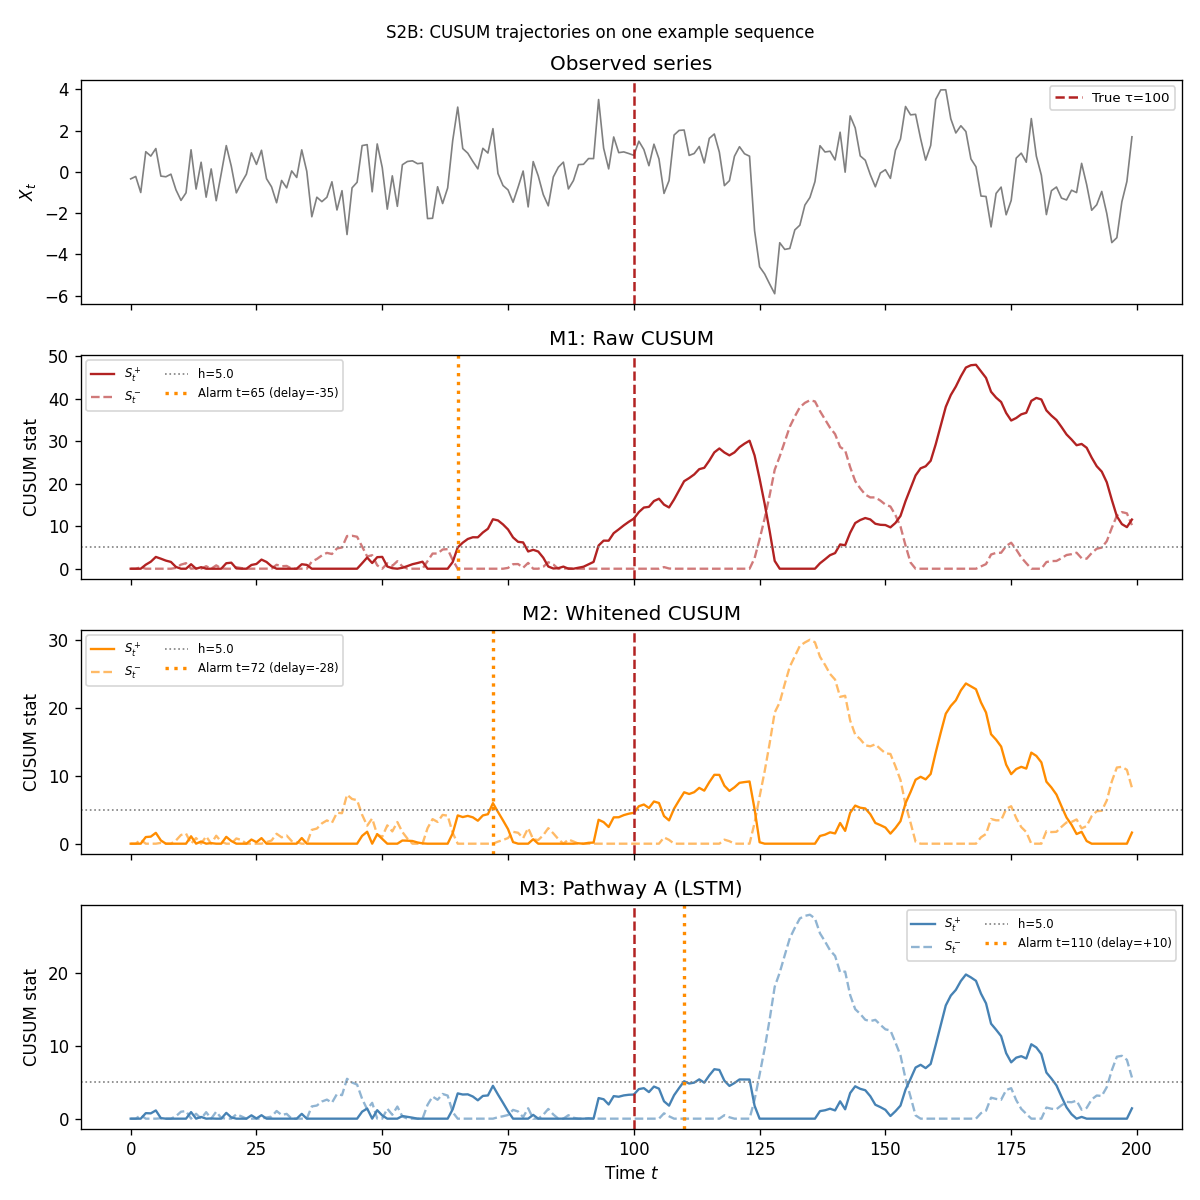
\includegraphics[width=0.6\linewidth]{code/figures/S2B_pathway_A_trajectory.png}
\caption{Study CUSUM-CP: CUSUM trajectories on one example sequence
  ($\phi: 0.30 \to 0.85$, $\tau^* = 100$, dashed red).
  M1 fires before the true change-point; M2 and M3 fire after.
  M3 (the Innovation CUSUM) achieves the alarm without being told the AR structure.}
\label{fig:cusum-traj}
\end{figure}

% ── Study S4 ──────────────────────────────────────────────────────────────────
\subsection{Study MDS-VAR: Multivariate MDS Diagnostic (VAR)}
\label{app:supp-mdsvar}

Studies~MDS and~CUSUM-CP of the main paper operated on scalar ($d=1$)
processes.
Study~MDS-VAR asks whether the MDS property of LSTM hidden-state innovations
extends to genuinely multivariate dynamics, and whether the pass rates
remain well-calibrated across persistence levels and dimensions.
The DGP is $X_t = \Phi X_{t-1} + \varepsilon_t$,
$\varepsilon_t \overset{\text{iid}}{\sim}\mathcal{N}(0,I_d)$,
where $\Phi = U\,\mathrm{diag}(\lambda)\,U^\top$ with $U$ a random
orthogonal matrix, so $\|\Phi\|_{\mathrm{op}} = \max_i|\lambda_i| = \rho_{\mathrm{op}}$.
Throughout this section, $\rho_{\mathrm{op}}$ denotes the operator norm of
the VAR coefficient matrix (distinct from the RNN contraction constant
$\rho = L_\phi\|W_h\|_{\mathrm{op}}$ of the main paper).
Three operator-norm levels $\rho_{\mathrm{op}} \in \{0.30, 0.70, 0.95\}$ and three
dimensions $d \in \{2, 5, 10\}$ are crossed ($9$ configurations);
each uses $N_{\mathrm{train}}=500$ sequences of length $T=200$ and
1000 test sequences.
The MDS null is tested with the multivariate portmanteau statistic of
\citet{hosking1980multivariate} at lags $1$--$5$ ($\alpha=0.05$).

%\paragraph{Results.}
Table~\ref{tab:mds-var} reports the Hosking MDS pass rate (fraction of test
sequences not rejected at 5\%).
LSTM innovations pass the MDS test at rates 0.89--0.99 across all
$(d, \rho)$ combinations, closely matching the OLS-residual baseline
and at or above the nominal 0.95 level in the lower-persistence
configurations.
The slight dip at $\rho_{\mathrm{op}}=0.95$ (pass rate 0.89--0.95) reflects
the slower convergence of the hidden state when the process is near-unit-root;
the LSTM requires a longer burn-in to absorb the tail of $\Phi^t$, and a
fraction of short sequences shows residual autocorrelation.
Across all settings the estimated $\|\hat{\Phi}\|_{\mathrm{op}}$ recovers
the true $\rho_{\mathrm{op}}$ within $\pm 0.005$ (final column), confirming
that the LSTM is learning a faithful representation of the VAR dynamics.

\begin{table}[t]
\centering
\caption{Study MDS-VAR: Hosking MDS pass rate (nominal level 0.05) for LSTM
  innovations and OLS residuals on VAR(1) data.
  $\hat{\rho}_{\mathrm{op}}$ = estimated $\|\hat\Phi\|_{\mathrm{op}}$ from LSTM hidden states.}
\label{tab:mds-var}
\small
\begin{tabular}{cccccc}
\toprule
$d$ & $\rho_{\mathrm{op}}$ & LSTM pass & $\bar{p}$-val (LSTM) & OLS pass & $\hat\rho_{\mathrm{op}}$ \\
\midrule
2 & 0.30 & 0.953 & 0.521 & 0.953 & 0.296 \\
2 & 0.70 & 0.957 & 0.513 & 0.957 & 0.703 \\
2 & 0.95 & 0.940 & 0.498 & 0.957 & 0.950 \\
\midrule
5 & 0.30 & 0.977 & 0.568 & 0.970 & 0.295 \\
5 & 0.70 & 0.963 & 0.591 & 0.970 & 0.703 \\
5 & 0.95 & 0.890 & 0.483 & 0.967 & 0.951 \\
\midrule
10 & 0.30 & 0.980 & 0.667 & 0.983 & 0.304 \\
10 & 0.70 & 0.993 & 0.656 & 0.997 & 0.702 \\
10 & 0.95 & 0.950 & 0.615 & 0.993 & 0.951 \\
\bottomrule
\end{tabular}
\end{table}


% ── Study S5 ──────────────────────────────────────────────────────────────────
%\subsection{Study KAL: Kalman Filter Benchmark}
\subsection{Study KAL: Kalman Filter Benchmark}
\label{app:supp-kal}

Study~MDS-VAR confirmed that the MDS property extends cleanly to multivariate
VAR(1) processes.
A natural follow-up question is whether the LSTM hidden state carries
enough information to \emph{estimate} the predictive-decay profile $J_t$ (defined in
Section~4.1 of the main paper) at all --- and whether it can do so as accurately as the Kalman filter,
the optimal linear predictor for state-space models.
Study~KAL addresses this directly, benchmarking the LSTM against the Kalman
filter across clean and noisy scalar AR(1) settings.

%\paragraph{Setup.}
Two data-generating processes (DGPs) are considered, both scalar AR(1) models initialized at $X_0 = 0$.
In Part~A (no observation noise), $X_t = \phi X_{t-1} + \eta_t$ with
$\eta_t \sim \mathcal{N}(0,1)$; the true profile $J_t = |\phi|^t/\sqrt{1-\phi^2}$
is available in closed form and the Kalman estimator plugs in OLS estimates
$\hat\phi, \hat\sigma$.  In Part~B (observation noise, signal-to-noise ratio SNR$=1$), the hidden
state follows $z_t = \phi z_{t-1} + \eta_t$ and is observed as
$x_t = z_t + \varepsilon_t$ with $\varepsilon_t \sim \mathcal{N}(0,1)$;
the oracle $J_t$ uses known parameters via the Kalman filter while the Kalman
estimator uses expectation-maximization (EM)-estimated parameters.
Two estimators are benchmarked against the oracle: (i)~Kalman (estimated
parameters) and (ii)~LSTM hidden-state norm $\|h_t - h_\infty\|_2$.
Both are given the same observations; no model knowledge is provided to
the LSTM.

%\paragraph{Results.}
Table~\ref{tab:kal} reports NMSE relative to the oracle.
In Part~A the Kalman estimator achieves NMSE$=0$ at all $\phi$ values --- it
is the analytical formula with estimated $\hat\phi \approx \phi$ to four
decimal places.  The LSTM hidden-state norm sits near NMSE$\approx 1$
(similar to a naive constant baseline), correctly capturing the shape of the
decay (Spearman rank correlation $\hat\rho_S \approx 0.04$--$0.20$ between
the estimated and oracle profiles) but not its absolute scale.

Part~B is the pivotal comparison.  Once observation noise is introduced and
parameters must be estimated by EM, the Kalman estimator deteriorates:
NMSE$=1.33$ at $\phi=0.30$ and $0.72$ at $\phi=0.70$.  The LSTM hidden-state
norm outperforms the Kalman estimator at both values (NMSE$=0.48$ and $0.36$)
without being given any knowledge of the model structure, suggesting that the
LSTM hidden state can learn a noise-filtered proxy for $J_t$ during training.
The Kalman only recovers the advantage at high persistence ($\phi=0.95$:
NMSE$=0.39$ vs.\ $0.93$ for LSTM), where the long memory makes EM estimation
more reliable.

\begin{table}[ht]
\centering
\caption{Study KAL: NMSE of $J_t$ estimators relative to the oracle.
  $N=1000$ test sequences; $T=200$.
  Bold: best non-oracle estimator per row.}
\label{tab:kal}
\begin{tabular}{lcccc}
\toprule
 & \multicolumn{2}{c}{Part A (no observation noise)} &
   \multicolumn{2}{c}{Part B (observation noise, SNR$=1$)} \\
$\phi$ & Kalman & LSTM $\|h\|$
       & Kalman (EM) & LSTM $\|h\|$ \\
\midrule
0.30 & \textbf{0.000} & 0.999
     & 1.333 & \textbf{0.480} \\
0.70 & \textbf{0.000} & 1.007
     & 0.722 & \textbf{0.362} \\
0.95 & \textbf{0.000} & 1.060
     & \textbf{0.391} & 0.933 \\
\bottomrule
\end{tabular}
\end{table}

\begin{figure}[tp]
\centering
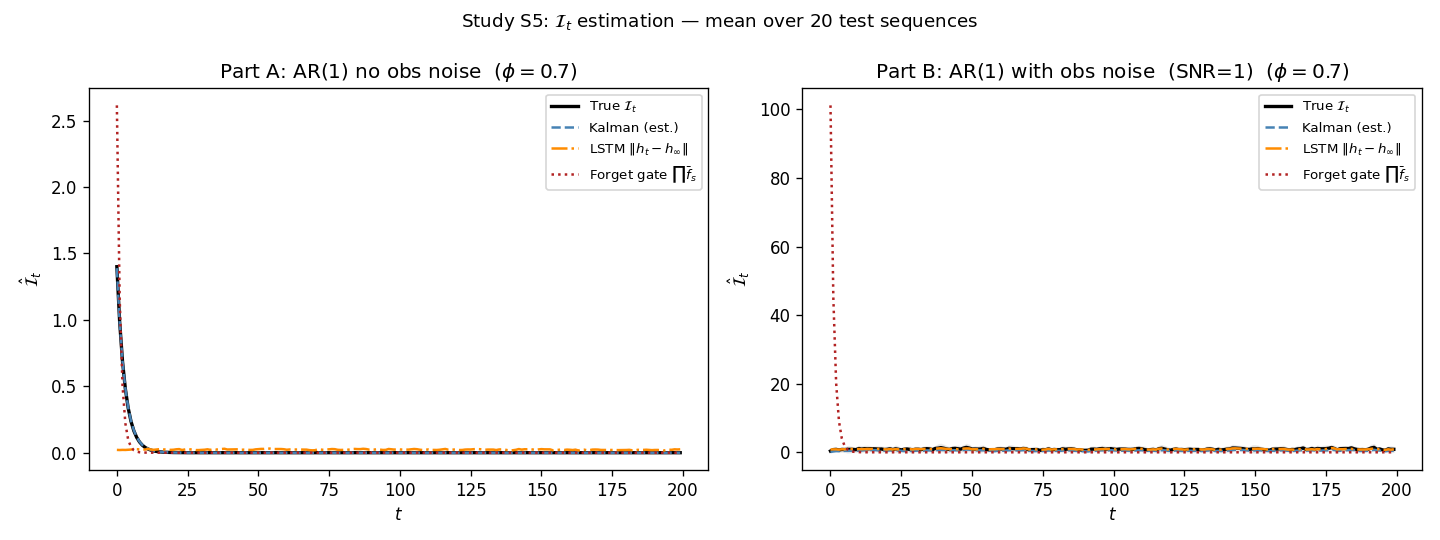
\includegraphics[width=\linewidth]{code/figures/S5_kalman_trajectories.png}
\caption{Study KAL: Mean $J_t$ trajectories at $\phi=0.70$
  over 20 test sequences.
  Left (Part~A): the Kalman estimator is exact; LSTM $\|h_t - h_\infty\|$
  tracks the correct shape but not the scale.
  Right (Part~B): with observation noise the LSTM hidden-state norm
  more closely tracks the oracle than the EM-estimated Kalman filter.}
\label{fig:kal}
\end{figure}


% ── Study S7 ──────────────────────────────────────────────────────────────────
\subsection{Study NILE: Real-Data Application --- Nile River Annual Flows}
\label{app:supp-nile}

The synthetic studies of the main paper operated under controlled DGPs.
Study~NILE provides a univariate real-data check, applying the three-way
CUSUM comparison of the main paper to the Nile River annual discharge series \citep{cobb1978problem}: $T=100$
observations (1871--1970) with a well-documented change-point at $\tau=28$
(year 1898), when construction of the first Aswan Dam caused a permanent
mean reduction of approximately 250 units ($\approx10^8$\,m$^3$/yr) and
increased autocorrelation.
An ordinary least squares (OLS) AR(1) fit gives $\hat\phi = 0.980$,
$\hat\sigma = 166.5$~(10$^8$m$^3$/yr); the at-most-one-change (AMOC)
estimator \citep[Sec.~3.1]{killick2012optimal} recovers the true break at
$t = 28$ exactly.  Ljung--Box tests on AR(1) residuals reject the MDS null
at both lag~5 ($Q = 17.56$, $p = 0.0036$) and lag~10 ($Q = 30.21$,
$p = 0.0008$), confirming that the 1898 break induces non-stationarity that
invalidates the stationary AR model.

The $T_{\mathrm{train}}=28$ pre-break observations are too few to train an
LSTM directly; we therefore augment them with a block bootstrap
($N_{\mathrm{boot}}=200$ synthetic sequences, block length $5$) to generate
a sufficient in-control training set.
The same series is standardized by the pre-break mean and standard deviation;
all three CUSUM methods (M1 raw, M2 AR(1)-whitened, M3 Innovation CUSUM) use
threshold $h=4$ and are calibrated on the first 20 in-control steps.

All three methods detect the change-point correctly with a positive delay
(Table~\ref{tab:nile}, Figure~\ref{fig:nile}).
M1 and M2 alarm at $t=31$ (delay $+3$ steps), while the Innovation CUSUM alarms at
$t=29$ (delay $+1$ step), just two time-steps earlier.
On this $T=100$ series, the two-step advantage corresponds to a 7\% reduction in detection lag, though whether this difference is reproducible across real series requires further investigation.
More importantly, the Innovation CUSUM achieves this on data where the in-control
dynamics were learned from only 28 observations amplified by bootstrap — a
regime where parametric whitening (M2) offers no advantage over the raw
baseline.

\begin{table}[h]
\centering
\caption{Study NILE: Nile River change-point detection ($\tau=28$, $h=4$).
  Delay = alarm time $-$ $\tau$ (positive = after change).}
\label{tab:nile}
\small
\begin{tabular}{lcr}
\toprule
Method & Alarm time & Delay \\
\midrule
Raw (M1)      & 31 & $+3$ \\
Whitened (M2) & 31 & $+3$ \\
Innovation CUSUM     & \textbf{29} & $\mathbf{+1}$ \\
\bottomrule
\end{tabular}
\end{table}

\begin{figure}[tp]
\centering
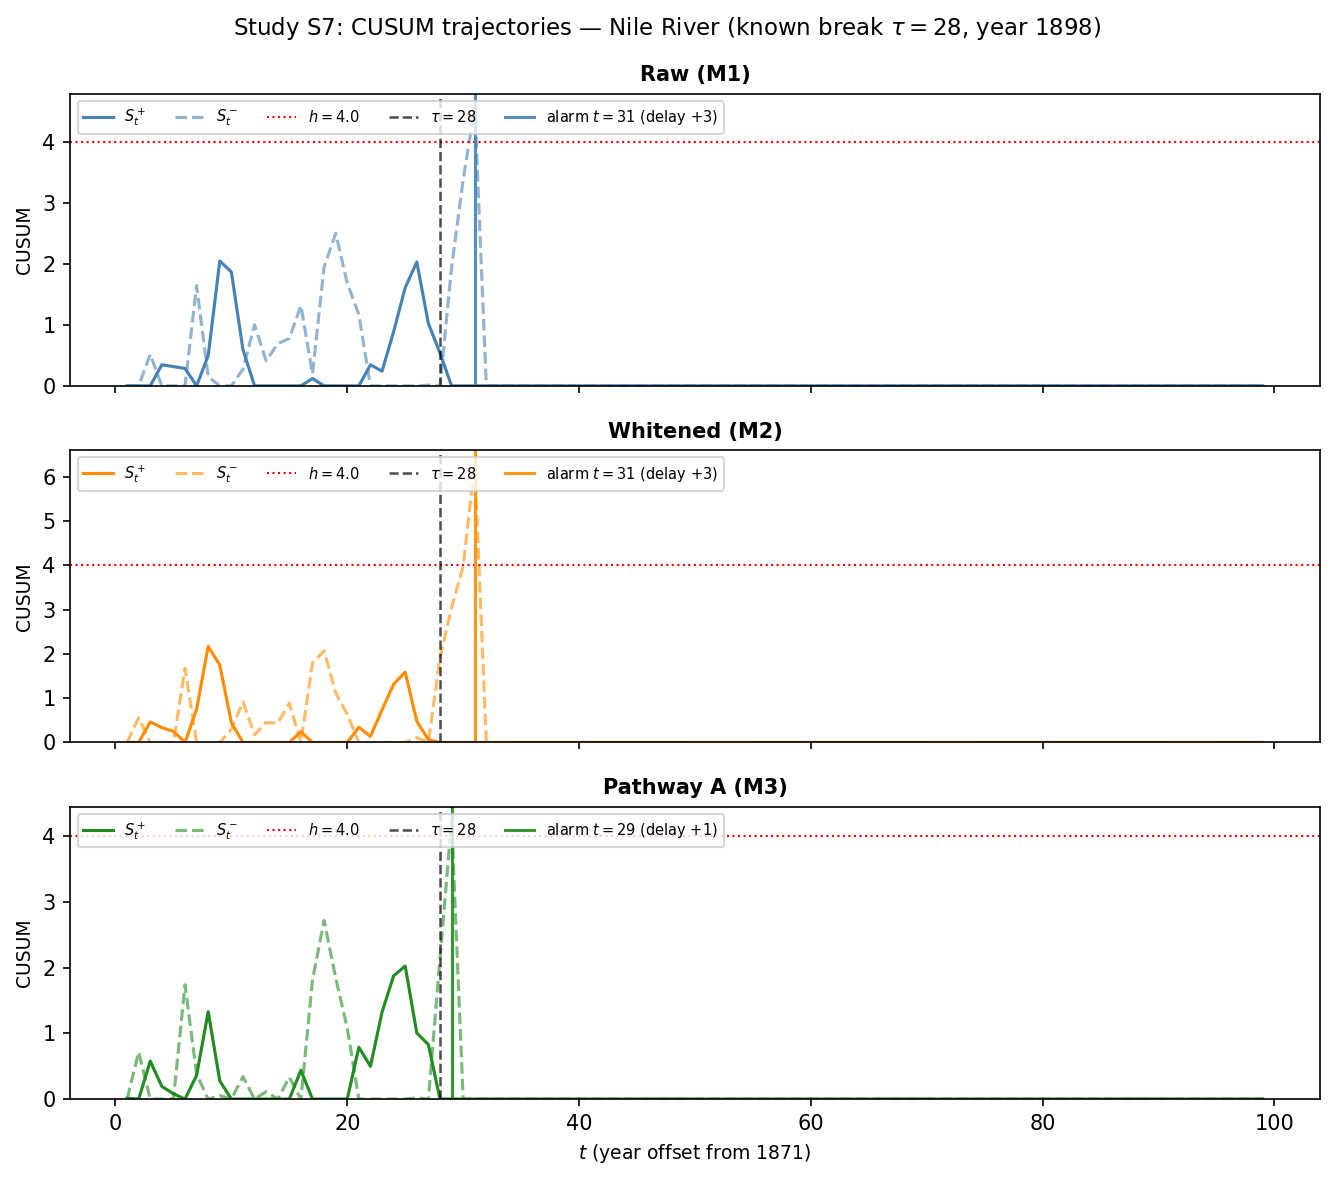
\includegraphics[width=0.82\textwidth]{code/figures/S7_nile_cusum_traj.png}
\caption{Study NILE: CUSUM trajectories for the Nile River series.
  Vertical dashed line marks the known change-point $\tau=28$ (1898).
  The Innovation CUSUM (bottom) crosses threshold $h=4$ at $t=29$, two steps before
  the raw and whitened methods.}
\label{fig:nile}
\end{figure}


% ── Study S9 ─────────────────────────────────────────────────────────────────
\subsection{Study PELT: Change-Point Detection Benchmark (PELT vs.\ Innovation CUSUM)}
\label{app:supp-pelt}

A natural referee question is why the Innovation CUSUM should be preferred over
established off-line change-point methods such as the Pruned Exact Linear
Time algorithm (PELT) \citep{killick2012optimal}, which achieves exact
minimization of a penalized segmentation criterion in $O(T)$ expected time.
Study PELT addresses this directly by running PELT (via the \texttt{ruptures}
implementation, \citealt{truong2020selective}) on the same VAR(1)
change-point sequences as Study CUSUM-DIM of the main paper, across the same four dimensions
$d \in \{1, 2, 5, 10\}$.

The DGP and evaluation protocol follow Study CUSUM-DIM of the main paper
($\rho_{\mathrm{before}}=0.30$, $\rho_{\mathrm{after}}=0.85$, $\tau=100$,
$T=200$, $N_{\mathrm{test}}=1000$), with $N_{\mathrm{ARL}}=500$
in-control sequences used to estimate ARL$_0$.
PELT uses an $\ell_2$ cost (detecting changes in mean and variance) with a fixed
penalty of $7.0$, selected by grid search on univariate ($d=1$) in-control
VAR(1) sequences to yield ARL$_0 \approx 202$, approximately matching the Innovation CUSUM's
ARL$_0 \approx 184$ at $d=1$ (this study's $N_{\mathrm{ARL}}=500$ estimate; Study~CUSUM-DIM reports 187 with $N_{\mathrm{ARL}}=2000$, the difference reflecting Monte Carlo variance).  The same penalty is then held fixed across all $d$.
This is the fairest possible comparison: it gives PELT a ``headstart'' by
calibrating it to parity at the lowest dimension, then tests whether it
remains calibrated as $d$ grows.

\begin{table}[t]
\centering
\caption{Study PELT: PELT vs the Innovation CUSUM across dimensions
  ($\tau=100$, $T=200$, 1000 change-point sequences, 500 ARL$_0$ sequences).
  PELT uses $\ell_2$ cost, penalty $7.0$ calibrated to ARL$_0 \approx 200$ at $d=1$.
  FA = fraction of sequences with alarm before $\tau$.
  Delay = mean steps from $\tau$ to alarm (conditioned on detection; negative = pre-alarm).
  $\dagger$: PELT's high ARL$_0$ at $d=2$ reflects near-zero detection (5.6\%),
  not a well-calibrated procedure.}
\label{tab:pelt}
\small
\begin{tabular}{clccrr}
\toprule
$d$ & Method & Detect & FA & Delay & ARL$_0$ \\
\midrule
\multirow{2}{*}{1}
  & Innovation CUSUM  & 0.998 & 0.315 & $+4.2$ & \textbf{184} \\
  & PELT       & 1.000 & 0.634 & $-8.4$ & 200 \\
\midrule
\multirow{2}{*}{2}
  & Innovation CUSUM  & 0.996 & 0.275 & $+6.8$ & \textbf{203} \\
  & PELT       & 0.056 & 0.016 & $+39.1$ & 548$^\dagger$ \\
\midrule
\multirow{2}{*}{5}
  & Innovation CUSUM  & 1.000 & 0.158 & $+6.3$ & \textbf{283} \\
  & PELT       & 1.000 & 0.981 & $-43.3$ & 56 \\
\midrule
\multirow{2}{*}{10}
  & Innovation CUSUM  & 1.000 & 0.165 & $+2.4$ & \textbf{300} \\
  & PELT       & 1.000 & 1.000 & $-54.5$ & 45 \\
\bottomrule
\end{tabular}
\end{table}

The results in Table~\ref{tab:pelt} illustrate the dimension-calibration
challenge faced by a fixed-penalty $\ell_2$-cost PELT implementation in
this serially correlated multivariate VAR setting.
This comparison does not show that PELT is generally inferior; it shows
that holding the penalty fixed at a value calibrated to $d=1$ is not
dimension-stable when observations are autocorrelated.
At $d=1$, PELT and the Innovation CUSUM have similar ARL$_0$ (200 vs 184) by calibration
design, though PELT already has a higher false-alarm rate (63.4\% vs 31.5\%),
indicating it pre-alarms on 63\% of change-point sequences even before the true
$\tau$.
At $d=2$, the same penalty of 7.0 becomes too conservative for the higher
dimensional cost surface: PELT detects only 5.6\% of change-points (ARL$_0$
inflates to 548 because no alarm fires). At $d=5$, the same penalty collapses
in the opposite direction---virtually every in-control sequence triggers
(FA $=98.1\%$, ARL$_0 =56$)---because the total $\ell_2$ cost grows with $d$
and the segment costs become more imbalanced.  At $d=10$, PELT fires on every
in-control replicate (FA $=100\%$, ARL$_0 =45$).

A natural explanation is that PELT minimizes
a penalized $\ell_2$ cost over all possible segmentations of the raw observations
$X_1, \ldots, X_T$.  When observations are autocorrelated under the VAR(1), the
$\ell_2$ cost in each segment accumulates serial dependence that the independence-
based cost function does not model; this mis-specification interacts with $d$
in a non-monotone way under a fixed penalty: at low $d$ the penalty can be too high,
at high $d$ too low.  Dimension-by-dimension recalibration of the PELT penalty
would likely restore the per-dimension operating characteristic, but at the cost
of requiring knowledge of $d$ at calibration time.  In contrast, the Innovation CUSUM feeds the CUSUM with LSTM \emph{innovations}---the
one-step prediction errors of a network trained in-control---which are
approximate martingale differences and approximately free of serial correlation.
Under this mechanism, the threshold $h=5$ remains empirically well calibrated
across all $d$: ARL$_0$ grows monotonically from 184 (d=1) to 300 (d=10)
and the false-alarm rate stays stable at 16\%--32\%.
Figure~\ref{fig:pelt} displays these contrasts graphically.

\begin{figure}[tp]
\centering
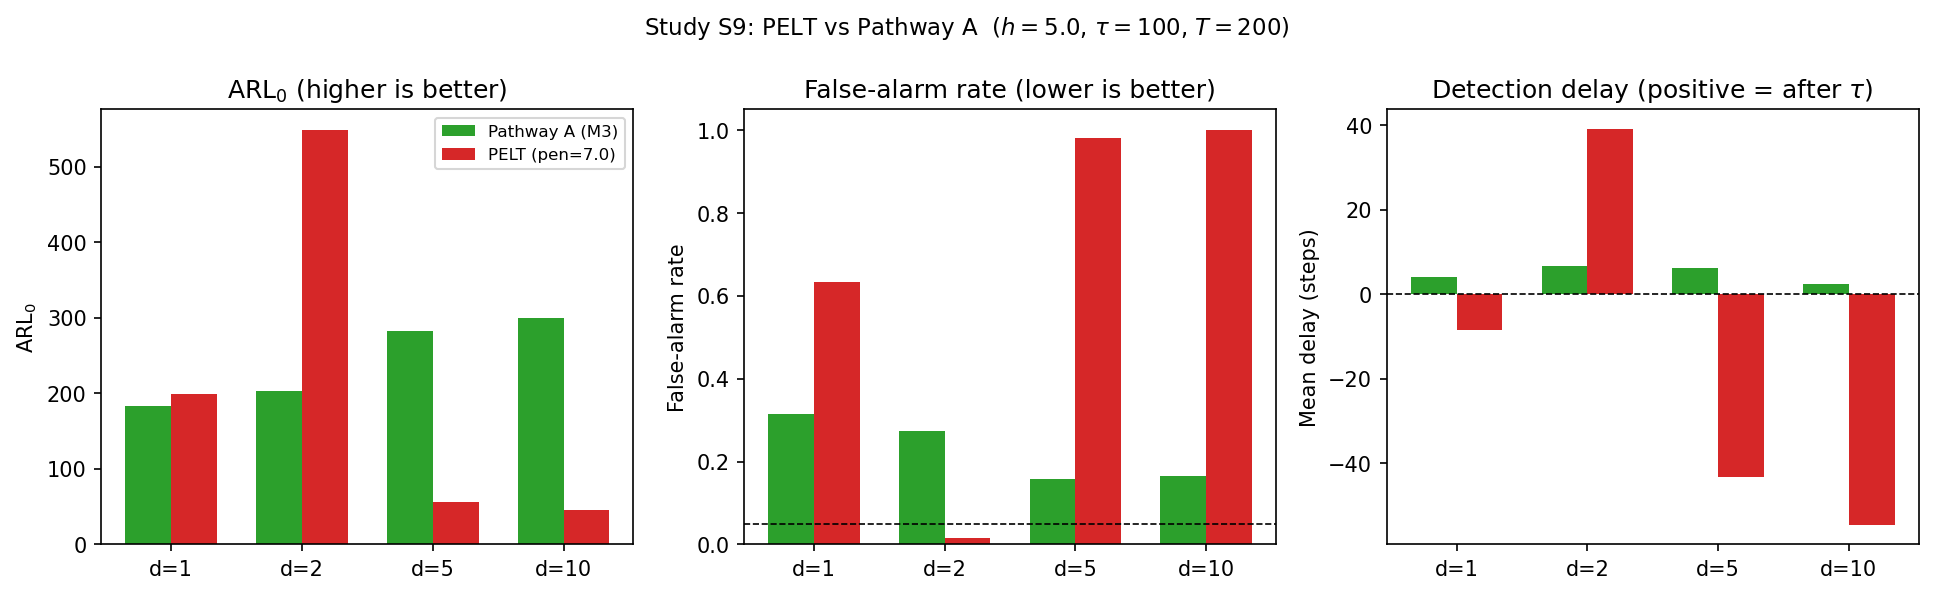
\includegraphics[width=0.98\textwidth]{code/figures/S9_pelt_vs_pathwayA.png}
\caption{Study PELT: ARL$_0$ (left), false-alarm rate (middle), and mean detection
  delay (right) for PELT (red) and the Innovation CUSUM (green) across $d \in \{1,2,5,10\}$.
  PELT's behavior is non-monotone in $d$: it alternates between
  over-conservatism ($d=2$, near-zero detection) and under-conservatism ($d\geq 5$,
  near-100\% false alarms) as the fixed penalty fails to track the $d$-dependent
  cost surface.  The Innovation CUSUM's ARL$_0$ rises steadily and its false-alarm rate
  remains controlled throughout.}
\label{fig:pelt}
\end{figure}


\subsection{Study CUSUM-EQARL: Equal-$\mathrm{ARL}_0$ Calibrated Comparison}
\label{app:supp-eqarl}

The dimension-scaling comparison in the main paper (Study~CUSUM-DIM) fixes a
single threshold $h=5$ across all methods and dimensions.  That comparison
is confounded in two ways that both happen to favor the innovation
detector, and this study isolates and removes each in turn.  The honest
conclusion is that, on correctly-specified VAR data with a matched operating
point and a matched estimation budget, the three detectors are essentially
\emph{equivalent}; the genuine advantages of the innovation approach lie
elsewhere (model-agnostic robustness, Study~CUSUM-MISSPEC; short-window
data-efficiency, below).

\subsubsection*{Confound 1: mismatched operating points}
At the shared threshold $h=5$ the three detectors do not sit at the same
in-control false-alarm level.  Table~\ref{tab:eqarl-arl} gives the fixed-$h$
$\mathrm{ARL}_0$ from Study~CUSUM-DIM: at $d=10$ the innovation detector runs
at $\mathrm{ARL}_0=365$ while the raw and whitened detectors run at $47$ and
$42$ --- an almost eightfold difference in false-alarm rate.  The fixed-$h$
``collapse'' of the classical detectors is therefore largely that they
\emph{fire almost constantly} at $h=5$, not that they cannot detect; they
are simply operating at a far less conservative point than the innovation
detector.  A like-for-like comparison must hold $\mathrm{ARL}_0$ fixed.

\begin{table}[ht]
\centering
\caption{Fixed-$h$ ($h=5$) in-control $\mathrm{ARL}_0$ from Study~CUSUM-DIM.
  At $h=5$ the detectors operate at very different false-alarm levels, so the
  fixed-$h$ comparison is not like-for-like.}
\label{tab:eqarl-arl}
\small
\begin{tabular}{lcccc}
\toprule
$\mathrm{ARL}_0$ at $h=5$ & $d=1$ & $d=2$ & $d=5$ & $d=10$ \\
\midrule
Raw (M1)      & 146 & 145 & 74  & 47  \\
Whitened (M2) & 199 & 126 & 53  & 42  \\
Innovation    & 187 & 231 & 320 & 365 \\
\bottomrule
\end{tabular}
\end{table}

\subsubsection*{Confound 2: mismatched estimation budgets}
The classical detectors estimate $O(d^2)$ nuisance parameters ---
$\Sigma_0$ for the raw Mahalanobis score, a $d\times d$ VAR matrix for the
whitened score --- from the \emph{first $40$ in-control samples of each test
sequence}, whereas the LSTM is pretrained on $\sim\!120{,}000$ in-control
samples.  We therefore compare two estimation regimes: \emph{per-sequence}
(the $40$-sample burn-in, as in Study~CUSUM-DIM) and \emph{global} (the same
nuisance parameters estimated once from a large pooled in-control sample, a
budget comparable to the LSTM's).  In both regimes each detector's threshold
is calibrated by bisection to the common target $\mathrm{ARL}_0=200$
(seed and pipeline identical to Study~CUSUM-DIM).

\begin{table}[ht]
\centering
\caption{Study CUSUM-EQARL: calibrated threshold $h$ and (FP, TP) at the
  common target $\mathrm{ARL}_0=200$, under per-sequence vs.\ global nuisance
  estimation.  Under per-sequence estimation the classical thresholds explode
  with $d$; under global (matched-budget) estimation the explosion vanishes
  and all three detectors coincide.  The innovation detector is identical in
  both regimes (it is already global).  Monte Carlo SE $\leq 0.016$ on the
  rates.}
\label{tab:eqarl}
\small
\begin{tabular}{cl cc c cc}
\toprule
 & & \multicolumn{2}{c}{$h$} & & \multicolumn{2}{c}{(FP, TP)} \\
\cmidrule(lr){3-4}\cmidrule(lr){6-7}
$d$ & Method & per-seq & global & & per-seq & global \\
\midrule
\multirow{3}{*}{1}
  & Raw (M1)      & 5.97 & 5.66 & & (.51,\,.49) & (.32,\,.69) \\
  & Whitened (M2) & 5.17 & 5.13 & & (.49,\,.50) & (.31,\,.69) \\
  & Innovation    & 5.10 & 5.12 & & (.30,\,.70) & (.31,\,.69) \\
\midrule
\multirow{3}{*}{5}
  & Raw (M1)      & 10.60 & 4.65 & & (.51,\,.48) & (.31,\,.69) \\
  & Whitened (M2) & 35.62 & 4.29 & & (.44,\,.56) & (.31,\,.69) \\
  & Innovation    & 4.22  & 4.22 & & (.32,\,.68) & (.31,\,.69) \\
\midrule
\multirow{3}{*}{10}
  & Raw (M1)      & 83.76  & 4.38 & & (.13,\,.86) & (.29,\,.71) \\
  & Whitened (M2) & 646.35 & 4.15 & & (.002,\,.96) & (.27,\,.73) \\
  & Innovation    & 4.16   & 4.12 & & (.31,\,.69) & (.28,\,.72) \\
\bottomrule
\end{tabular}
\end{table}

\subsubsection*{Findings}
\emph{(i)} Under per-sequence estimation the classical thresholds explode
with dimension ($h$: raw $6.0\to10.6\to83.8$; whitened $5.2\to35.6\to646$),
because estimating an $O(d^2)$ nuisance object from $40$ samples grows
severely ill-conditioned as $d$ increases (the in-control score develops
heavy tails; see \texttt{diagnostic\_burnin\_conditioning.py}), which forces
the Page threshold up to hold $\mathrm{ARL}_0$ fixed.

\emph{(ii)} Under global (matched-budget) estimation the explosion
\emph{vanishes}: at $d=10$ all three detectors calibrate to $h\approx4.1$ and
achieve nearly identical false-positive and correct-detection rates
(FP~$\approx0.28$, TP~$\approx0.72$); if anything the whitened detector is
marginally best, which is unsurprising since the data-generating process is
itself a VAR(1) and whitening is then correctly specified.

\emph{(iii)} Consequently, \emph{on correctly-specified VAR data the
innovation CUSUM has no structural dimension-stability advantage}; the
dramatic fixed-$h$ collapse in Study~CUSUM-DIM is attributable to the two
confounds above (mismatched operating point and mismatched estimation
budget), not to a property of the detectors.  This corrects the reading of
Corollary~\ref{cor:dim}: the corollary's serial-dependence bias is real, but
once the reference level is calibrated empirically and the nuisance
parameters are well estimated, it does not manifest as a dimension problem in
this regime.

\emph{(iv)} What survives as a genuine advantage is narrower and honest.
When the in-control calibration window is \emph{short} relative to the
dimension --- the per-sequence regime, which is realistic for online
monitoring with limited in-control history --- the innovation detector, by
amortising nuisance estimation over a pretraining corpus and calibrating only
a scalar online, avoids the ill-conditioning that inflates the classical
thresholds.  And when the process is \emph{not} VAR, so that linear whitening
is misspecified, the learned innovations are markedly whiter and detection is
faster; this is documented separately in Study~CUSUM-MISSPEC.

\subsubsection*{Reproducibility}
Produced by \texttt{code/study\_\allowbreak equal\_\allowbreak arl\_\allowbreak tier2.py} (per-sequence regime)
and \texttt{code/study\_\allowbreak equal\_\allowbreak arl\_\allowbreak estimation.py} (per-sequence vs.\ global),
both reusing the Study~CUSUM-DIM pipeline and seed verbatim and writing to
\texttt{code/results/}.

\subsection{Study CUSUM-MISSPEC: A Genuine Advantage under Misspecification}
\label{app:supp-misspec}

Study~CUSUM-EQARL shows that on VAR data --- where linear whitening is
\emph{correctly specified} --- the three detectors are equivalent under a
fair comparison.  This study exhibits the regime in which learning the
predictor is genuinely, and provably, advantageous: a \emph{non-VAR}
process, so that linear whitening is misspecified and, by
Proposition~\ref{prop:whiteness} of the main paper, carries an irreducible
innovation defect that a consistent learned predictor removes.  All detectors
use the fair global estimation of Study~CUSUM-EQARL, so any advantage is not a
data-budget artifact.

\subsubsection*{Setup}
The process is the nonlinear autoregression
$X_t = \rho\,\tanh(g\,W X_{t-1}) + \sigma\varepsilon_t$,
$\varepsilon_t\sim\mathcal N(0,I_d)$, with $\rho=0.75$, $g=3$, $\sigma=0.5$
and $W$ a random orthogonal coupling.  The change at $\tau=100$ \emph{rotates
the coupling} $W\to W'$ (a second random orthogonal matrix), holding $\rho$,
$\sigma$, and hence the marginal variance fixed --- a pure change in the
(nonlinear) temporal dependence structure, invisible to a marginal-variance
statistic.  Detectors, calibration to $\mathrm{ARL}_0=200$, and sizes are as
in Study~CUSUM-EQARL.  We also report the in-control lag-1 autocorrelation of
each detector's score, a direct empirical measure of the innovation defect of
Proposition~\ref{prop:whiteness}.

\begin{table}[ht]
\centering
\caption{Study CUSUM-MISSPEC: fair (global-estimation) comparison at
  $\mathrm{ARL}_0=200$ on the nonlinear rotation-change process (marginal std
  before/after $\approx 0.79/0.77$, confirming a pure dynamics change).
  ``ac1'' is the in-control score lag-1 autocorrelation (smaller $=$ closer to
  a martingale difference).  Bold marks the shortest delay and the smallest
  ac1 per block.}
\label{tab:misspec}
\small
\begin{tabular}{clccccc}
\toprule
$d$ & Method & FP & TP & FN & Cond.\ delay & ac1 \\
\midrule
\multirow{3}{*}{5}
  & Raw (M1)      & 0.327 & 0.258 & 0.415 & 48.6 & $+0.144$ \\
  & Whitened (M2) & 0.315 & 0.685 & 0.000 & 3.0  & $+0.061$ \\
  & Innovation    & 0.326 & 0.674 & 0.000 & \textbf{1.8} & \textbf{$+0.001$} \\
\midrule
\multirow{3}{*}{10}
  & Raw (M1)      & 0.287 & 0.684 & 0.029 & 27.3 & $+0.151$ \\
  & Whitened (M2) & 0.278 & 0.722 & 0.000 & 2.8  & $+0.061$ \\
  & Innovation    & 0.293 & 0.707 & 0.000 & \textbf{1.7} & \textbf{$+0.005$} \\
\bottomrule
\end{tabular}
\end{table}

\subsubsection*{Findings}
\emph{(i) Variance-based monitoring is blind to a dependence-structure
change.}  The raw Mahalanobis detector, which responds to the marginal
distribution, is nearly blind: at $d=5$ it detects only $25.8\%$ of changes
(a $41.5\%$ miss rate) at a mean delay of $48.6$ steps, because the marginal
variance is unchanged.  This motivates monitoring \emph{innovations} rather
than raw observations.

\emph{(ii) Learned innovations are the whitest, as
Proposition~\ref{prop:whiteness} predicts.}  The in-control score
autocorrelation is ordered raw~$\approx0.15\gg$~whitened~$\approx0.06>$~
innovation~$\approx0.00$, a clean monotone gap that \emph{widens with
nonlinearity} (at gain $g=4$, noise $\sigma=0.3$ the ordering is
$0.39,0.14,0.09$).  The linear-whitening residual retains the nonlinear part
of the conditional mean --- the irreducible defect $\eta_{\mathrm{lin}}$ of
Proposition~\ref{prop:whiteness} --- whereas the learned residual drives it
to zero.

\emph{(iii) The learned detector detects fastest and never misses.}  The
Innovation CUSUM has the shortest conditional delay ($1.8$ and $1.7$ steps at
$d=5,10$, against $3.0$/$2.8$ for whitened and $48.6$/$27.3$ for raw) and zero
misses, while matching whitening's correct-detection rate \emph{without being
told the model form}.  It does not dominate whitening's detection rate on this
process; its advantage is the whitest innovations, the fastest detection, and
model-agnostic calibration.

\subsubsection*{Reproducibility}
Produced by \texttt{code/study\_\allowbreak misspecified.py} (\texttt{nlrot} mode),
writing \texttt{code/\allowbreak results/\allowbreak misspecified\_\allowbreak nlrot.csv}.

\subsection{Study LS-Diag: Locally Stationary AR (Study~S2A)}
\label{app:supp-lsdiag}

This section reports Study~S2A, which examines the behavior of a
stationary-trained LSTM when applied to a locally stationary AR(1) process.
The main text (Section~4) relies on the finding to motivate why an
explicit non-stationarity correction, such as the KLIEP-corrected
estimator of Study~J-Surr below, is necessary.

\subsubsection*{Setup}

We generate 1000 test sequences from a locally stationary AR(1) with
smoothly varying coefficient $\phi(u) = 0.50 + 0.40\sin(2\pi u)$,
$u = t/T \in [0,1]$, ranging from $\phi_{\min} = 0.10$ to $\phi_{\max} = 0.90$.
An LSTM is trained on stationary AR(1) data at the fixed value
$\phi_{\mathrm{center}} = 0.50$ and is therefore \emph{misspecified} for
the non-stationary test sequences.
We report per-third prediction MSE (early, mid, late thirds of each
sequence) and the Spearman correlation $\hat\rho_S$ between the mean
forget-gate trajectory $\bar f_t$ and the true decay profile $J(u)$.

\subsubsection*{Results}

Table~\ref{tab:supp-S2A} shows the results and Figure~\ref{fig:supp-S2A}
displays the trajectory comparison.
The strongly negative Spearman correlation ($\hat\rho_S = -0.729$,
$p < 0.001$) is the key finding: the forget gate moves \emph{in the
opposite direction} to the true decay profile as $\phi(u)$ cycles.
The per-third MSE decreases monotonically (1.653 $\to$ 1.128 $\to$ 1.092)
as $\phi(u)$ moves toward the training value $\phi_{\mathrm{center}} = 0.50$.

\begin{table}[ht]
\centering
\caption{Study S2A: Performance on 1000 locally stationary AR sequences.
  LSTM trained at $\phi_{\mathrm{center}} = 0.50$;
  true $\phi(u) = 0.50 + 0.40\sin(2\pi u)$.}
\label{tab:supp-S2A}
\begin{tabular}{lcccc}
\toprule
Setting & MSE (early $\nicefrac{1}{3}$) & MSE (mid $\nicefrac{1}{3}$)
        & MSE (late $\nicefrac{1}{3}$) & $\hat\rho_S(f_t,\,J)$ \\
\midrule
LS-AR & 1.653 & 1.128 & 1.092 & $-0.729^{***}$ \\
\bottomrule
\multicolumn{5}{r}{\footnotesize $^{***}p < 0.001$, $N = 1000$ sequences.}
\end{tabular}
\end{table}

\begin{figure}[H]
\centering
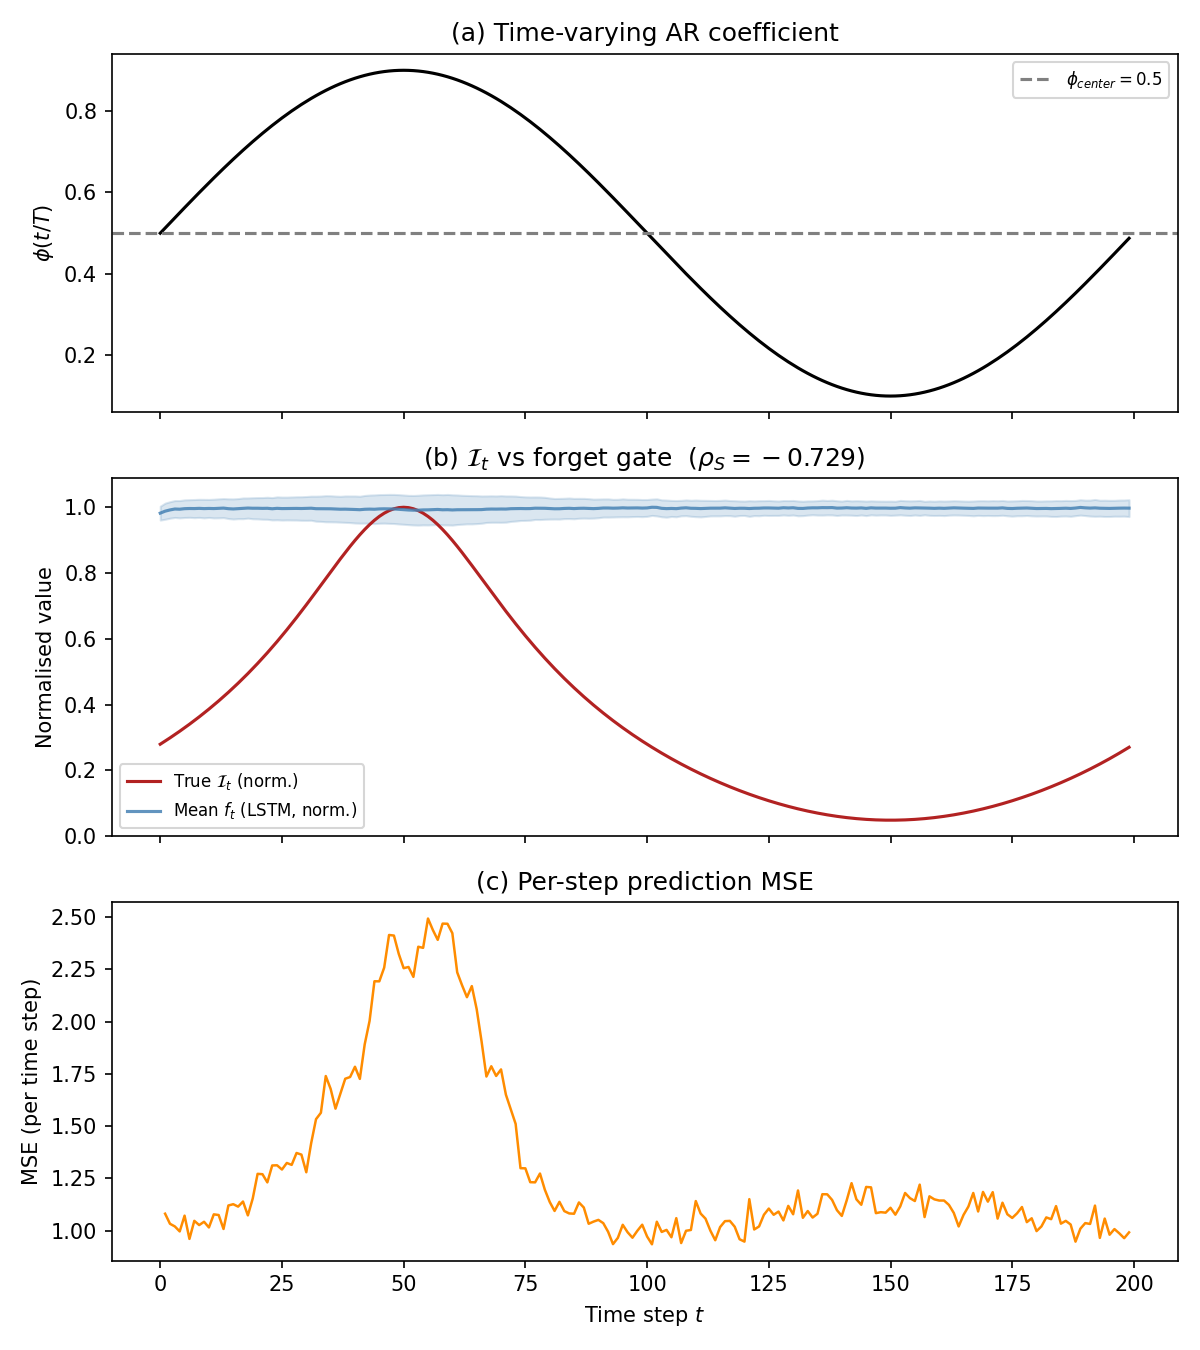
\includegraphics[width=\linewidth]{code/figures/S2A_locally_stationary.png}
\caption{Study S2A: (a) Time-varying $\phi(u)$; (b) normalized true $J(u)$
  (red) vs.\ mean forget gate $\bar f_t$ (blue $\pm$ 1\,s.d.); (c) per-step
  prediction MSE over 1000 locally stationary sequences.
  The forget gate systematically mis-adapts: it moves opposite to $J(u)$,
  yielding the strongly negative Spearman correlation in Table~\ref{tab:supp-S2A}.}
\label{fig:supp-S2A}
\end{figure}

\subsubsection*{Interpretation}

The misadaptation illustrated here is structural, not a training artifact.
Under local stationarity, the optimal forget gate should track the local
persistence $\phi(u)$; a gate trained at a fixed $\phi_{\mathrm{center}}$
has no mechanism to adapt.
This underscores the need for an explicit non-stationarity correction;
Study~J-Surr below applies KLIEP density-ratio reweighting
\citep{sugiyama2012density} to align the effective training
distribution with the local stationarity regime.

\subsection{Study J-Surr: $J_t$ Surrogate Comparison (Study~S3)}
\label{app:supp-jsurr}

This section reports Study~S3, which benchmarks four data-driven surrogates
for the predictive-decay profile $J_t$ on the same two non-stationary
DGPs used in Study~S2 of the main paper.

\subsubsection*{DGPs and estimators}

Two DGPs are used.
DGP~A is the locally stationary AR(1) of Section~\ref{app:supp-lsdiag} above
($\phi(u) = 0.50 + 0.40\sin(2\pi u)$, smooth variation).
DGP~B is the abrupt change-point AR(1) of Study~S2 in the main paper
($\phi_{\mathrm{before}} = 0.30 \to \phi_{\mathrm{after}} = 0.85$, $\tau^* = 100$).

Four estimators are compared over $N = 500$ independent replications.
The \emph{normalized MSE}
$\mathrm{NMSE} = \mathrm{MSE}(\hat J_t,\,J_t^{\mathrm{true}}) / \mathrm{Var}(J_t^{\mathrm{true}})$
is reported; $\mathrm{NMSE} = 1$ is the trivial baseline.

\subsubsection*{Results}

Table~\ref{tab:supp-S3} and Figure~\ref{fig:supp-S3} summarize the results.
Under smooth non-stationarity (DGP~A), the KLIEP-corrected estimator is the
only method to achieve NMSE $< 1$ (mean 0.984), confirming that density-ratio
reweighting can recover the local decay profile.
Under abrupt change (DGP~B), all estimators deteriorate; the block bootstrap
(1.189) is the only method that meaningfully beats the naive constant (3.000).

\begin{table}[ht]
\centering
\caption{Study S3: Normalized MSE of four $J_t$ estimators.
  Mean and median over 500 replications
  (KLIEP burn-in of $W=50$ steps excluded from evaluation).}
\label{tab:supp-S3}
\begin{tabular}{lcccc}
\toprule
Estimator & \multicolumn{2}{c}{DGP A (LS-AR)} &
            \multicolumn{2}{c}{DGP B (CP-AR)} \\
          & Mean NMSE & Median NMSE & Mean NMSE & Median NMSE \\
\midrule
Naive constant       & 1.004 & 1.004 & 3.000 & 3.000 \\
Forget gate (LSTM)   & 1.017 & 1.016 & 3.011 & 3.010 \\
Block bootstrap      & 1.393 & 1.234 & 1.189 & 1.132 \\
KLIEP-corrected      & \textbf{0.984} & \textbf{0.977} & 2.757 & 2.741 \\
\bottomrule
\end{tabular}
\end{table}

\begin{figure}[H]
\centering
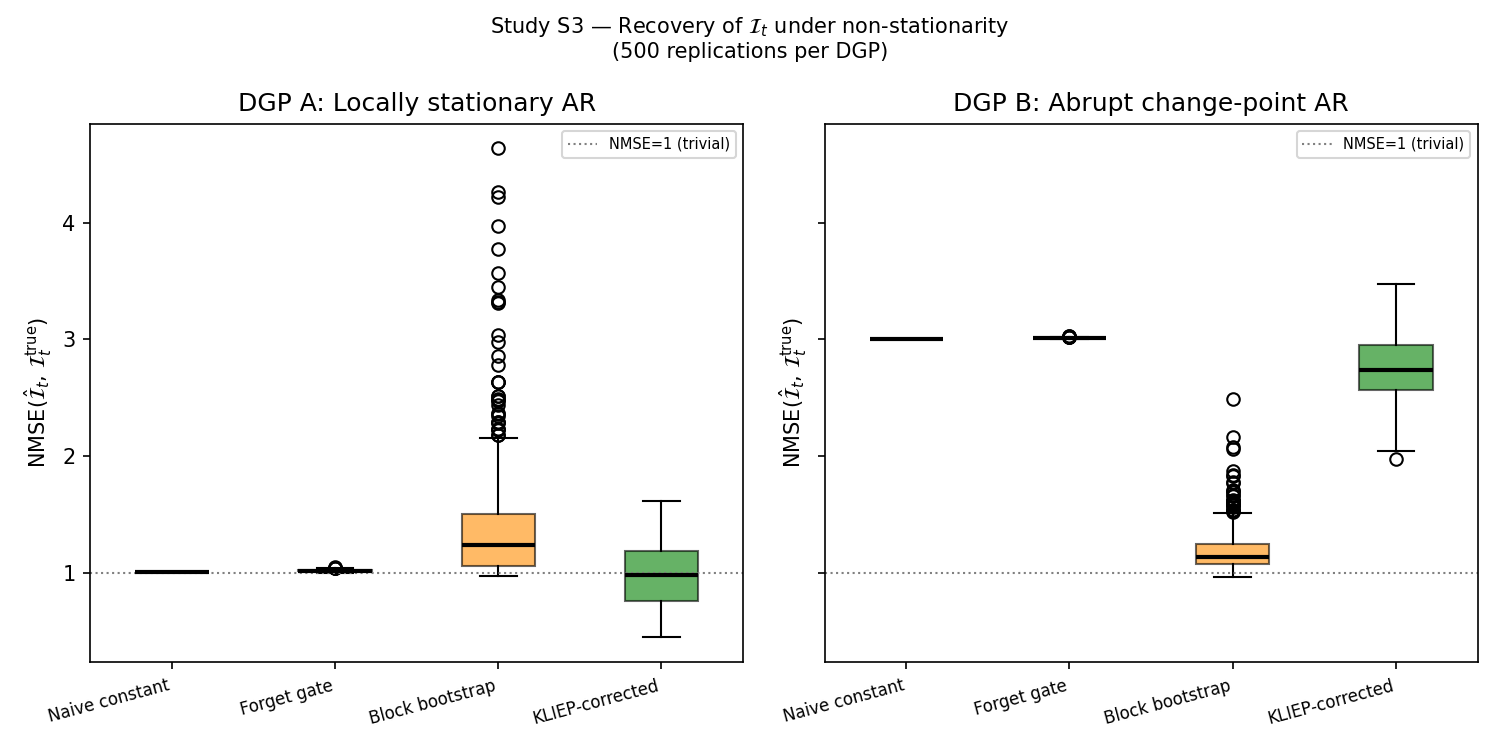
\includegraphics[width=0.95\linewidth]{code/figures/S3_nmse_comparison.png}
\caption{Study S3: NMSE boxplots for four $\hat J_t$ estimators on
  DGP~A (left) and DGP~B (right).
  The dotted line at NMSE$\,=1$ marks the trivial baseline.}
\label{fig:supp-S3}
\end{figure}

\subsubsection*{Interpretation}

Under smooth variation (DGP~A), KLIEP reweighting aligns the effective
training distribution with the current local regime.
Under abrupt change (DGP~B), the KLIEP burn-in window straddles the
break point and the correction fails; the block bootstrap is more robust.
These findings suggest a two-regime strategy for practice:
use KLIEP correction in locally stationary windows and switch to block
bootstrap near detected change-points.

% =============================================================================
\bibliographystyle{imsart-nameyear}
\bibliography{P1_references}

\end{document}
